\documentclass[../main.tex]{subfiles}
\begin{document}
%%%%%%%%%%%%%%%%%%%Seven types %%%%%%%%%%%%%%%%%%%%%%%%%%%
% \chapter{Dynamic Programming Questions}
In this Chapter, we categorize dynamic programming into three according to the input data types, including Single Sequence (Section~\ref{sec_single_n} and Section~\ref{sec_single_n2}), Coordinate (Section~\ref{sec_coordinate}), and Double Sequence(Section~\ref{sec_double_sequence}). Each type has its own identifiable characters and can be solved in a certain similar way. In this process, we found the \textbf{Forward Induction Method} is the most effective way to identify the recurrence state transfer function.  In Forward Induction Method, we start from the base cases (corresponds to the base cases in the DFS solution), and incrementally move to the larger subproblem, and try to induce the state transfer function between current problem and its previous subproblems. If can be induced from only constant subproblems, we have $O(n)$, if relates to all smaller subproblems, we have $O(n^2)$. Using forward inductio method, is intuitive and effective. The only thing we need to note is to try a variety of examples, make sure the recurrence function we found is comprehensive and right.  At the end of the section, we would summarize a template for this type of problems solved using dynamic programming. These types include:
\begin{enumerate}
    \item Single Sequence (50\%):  This is an easy type too. The states represents if the sequence ends here and include the current element. This way of divide the problem we can obtain the state transfer function easily to find a pattern. 
    \item Coordinate (15\%): 1D or 2D coordinate. This is the easiest type of DP because the state transfer function can be directly obtained through the problem (how to make moves to the next position). 
    \item Double Sequence (30\%): Because double sequence make its state a matrix and subproblem size $O(mn)$, this type of dynamic programming is similar to coordinate type, within which we just need to figure out the transfer function (moves) ourselves. 
    % \item Splitting Type (10\%): The splitting type is quite different in the ways of dividing the problem. 
    % \item Backpack Type (10\%):
    % \item Range Type (10\%):
\end{enumerate}
    % 坐标型15%: jump game: 棋盘,格子 f[i]代表从起点走到i坐标
    % 序列型30%:f[i]代表前i个元素总和,i=0表示不取任何元素
    % 双序列型30%
    % 划分型10%
    % 背包型10%
    % 区间型5%
%%%%%%%%%%%%%%%%%%%single sequence %%%%%%%%%%%%%%%%%%%%%%%%%%%
% \section{Single Sequence}
% \label{part2_sequence_dp}
The single sequence type dynamic programming is usually applied on the string and array. 
\begin{table}[h]
\begin{small}
\centering
\noindent\captionof{table}{ Different Type of Single Sequence Dynamic Programming}
 \noindent \begin{tabular}{|p{0.14\columnwidth}|p{0.14\columnwidth}| p{0.14\columnwidth}|p{0.14\columnwidth}|p{0.14\columnwidth}|p{0.14\columnwidth}|}
  \hline
 Case & Input & Subproblems & f(n) & Time & Space   \\ \hline
Section~\ref{sec_single_n}  & $O(n)$& $O(n)$ & $O(1)$ & $O(n)$ & $O(n)->O(1)$ \\\hline
Section~\ref{sec_single_n2}  & $O(n)$& $O(n)$ & $O(n)$ & $O(n^2)$ & $O(n)$\\ \hline
Section~\ref{sec_single_n3}  & $O(n)$& $O(n^2)$ & $O(n)$ & $O(n^3)$ & $O(n^2)$\\ \hline
Hard  & $O(n)$& $O(n^3)$ & $O(n)$ & $O(n^4)$ & $O(n^3)$\\ \hline
\end{tabular}
  \label{tab:single_sequence}
  \end{small}
\end{table}

\begin{table}[h]
\begin{small}
\centering
\noindent\captionof{table}{ Different Type of Coordinate Dynamic Programming}
 \noindent \begin{tabular}{|p{0.14\columnwidth}|p{0.14\columnwidth}| p{0.14\columnwidth}|p{0.14\columnwidth}|p{0.14\columnwidth}|p{0.14\columnwidth}|}
  \hline
 Case & Input & Subproblems & f(n) & Time & Space   \\ \hline
Easy  & $O(mn)$& $O(mn)$ & $O(1)$ & $O(mn)$ & $O(mn)->O(m)$ \\\hline
Medium  & $O(mn)$& $O(kmn)$ & $O(1)$ & $O(kmn)$ & $O(kmn)->O(mn)$\\ \hline
\end{tabular}
  \label{tab:2d_coordinate}
  \end{small}
\end{table}

% \begin{enumerate}
%     \item     state: $f[i]$ denotes the state for number or character for the first $i$ position, or the $i$th. Normally need $n+1$ space, because we need to consider the empty string; 
%     \item    function: $f[i] = f[j]$ … $j$ is the position previous to $i$; 
%     \item initialize: $f[0]$
%     \item answer: $f[n]$, while not $n-1$; 
% \end{enumerate}


Now, let us look at some examples: 
%%%%%%%%%%%%%%%%%%%%%%%%%%%%%%%%%%%%%Single Sequence%%%%%%%%%%%%%%%%%%%
\section{Single Sequence $O(n)$}
\label{sec_single_n}
In this section, we will see how to solve the easy type of dynamic programming shown in Table~\ref{tab:single_sequence}, where each subproblem is only dependent on the state of constant number of smaller subproblems. \textbf{Subarray} and \textbf{Substring} are two types of them. Here, we will see how to using \textit{deduction} method which starts from base case, and gradually get the result of all the cases after it. The examples include probelems with one or multiple choice.

Moreover, for this type, because for each subproblem, we only need to look back constant smaller subproblems, we do not even need $O(n)$ space to save all the result, unless you are asked to get the best solution for all subproblems too. Thus, this section generally achieve $O(n)$ and $O(1)$ for time complexity and space complexity, respectively. 
\begin{enumerate}
    \item 276. Paint Fence
    \item 256. Paint House
    \item 198. House Robber
    \item 337. House Robber III (medium)
    \item 53. Maximum Subarray (Easy) 
    \item 152. Maximum Product Subarray
    \item 32. Longest Valid Parentheses(hard)
\end{enumerate}
\subsection{Easy Type}
\begin{examples}
\item \textbf{Paint Fence (L276, *).} There is a fence with n posts, each post can be painted with one of the k colors. You have to paint all the posts such that no more than two adjacent fence posts have the same color.Return the total number of ways you can paint the fence. \textit{Note: n and k are non-negative integers.}
\begin{lstlisting}[numbers=none]
Example:

Input: n = 3, k = 2
Output: 6
Explanation: Take c1 as color 1, c2 as color 2. All possible ways are:

            post1  post2  post3      
 -----      -----  -----  -----       
   1         c1     c1     c2 
   2         c1     c2     c1 
   3         c1     c2     c2 
   4         c2     c1     c1  
   5         c2     c1     c2
   6         c2     c2     c1
\end{lstlisting}
\textbf{Solution: Induction and Multi-choiced State}. suppose n=1, dp[1] = k; when n=2, we have two cases: same color with k ways to paint and different color with k*(k-1) ways. 
\begin{lstlisting}[numbers=none]
dp[1] = k
dp[2] = same + diff; same = k, diff = k*(k-1)
dp[3]: for dp[2].same, we can only have diff colors, diff = dp[2].same*(k-1)
       for dp[2].diff, we can have either diff color or small  color, same = dp[2].diff, diff+=dp[2].diff*(k-1)
\end{lstlisting}
Thus, using deduction, which is the dynamic programming, the code is:
\begin{lstlisting}[language=Python]
def numWays(self, n, k):
    if n==0 or k==0:
        return 0
    if n==1:
        return k
    
    same = k
    diff = k*(k-1)
    for i in range(3,n+1):
        pre_diff = diff
        diff = (same+diff)*(k-1)
        same = pre_diff
    return (same+diff)
\end{lstlisting}
\item \textbf{Paint House (L256, *).} There are a row of n houses, each house can be painted with one of the three colors: red, blue or green. The cost of painting each house with a certain color is different. You have to paint all the houses such that no two adjacent houses have the same color.

The cost of painting each house with a certain color is represented by a n x 3 cost matrix. For example, costs[0][0] is the cost of painting house 0 with color red; costs[1][2] is the cost of painting house 1 with color green, and so on... Find the minimum cost to paint all houses. \textit{Note: All costs are positive integers.}
\begin{lstlisting}[numbers=none]
Example:

Input: [[17,2,17],[16,16,5],[14,3,19]]
Output: 10
Explanation: Paint house 0 into blue, paint house 1 into green, paint house 2 into blue. 
             Minimum cost: 2 + 5 + 3 = 10.

\end{lstlisting}
\textbf{Solution: Induction and Multi-choiced State.} For this problem, each item has three choice, so we need to track the optimal solution for taking each color. dp[0] = 0, for one house, return min(c1, c2, c3). 
\begin{lstlisting}[numbers=none]
for 1 house: for three choice - (c1, c2, c3), the result is min(c1, c2, c3)
for 2 houses: cost of taking c1 = costs[2][c1]+min(dp[1].c2, dp[1].c3)
              cost of taking c2 = costs[2][c2]+min(dp[1].c1, dp[1].c3)
              cost of taking c3 = costs[2][c3]+min(dp[1].c1, dp[1].c2)
\end{lstlisting}
\begin{lstlisting}[language=Python]
def minCost(self, costs):
    if not costs:
        return 0
    c1, c2, c3 = costs[0]
    n = len(costs)
    for i in range(1, n):
        nc1 = costs[i][0] + min(c2, c3)
        nc2 = costs[i][1] + min(c1, c3)
        nc3 = costs[i][2] + min(c1, c2)
q        c1, c2, c3 = nc1, nc2, nc3
    return min(c1, c2, c3)
\end{lstlisting}
\item \textbf{House Robber (L198,*).} You are a professional robber planning to rob houses along a street. Each house has a certain amount of money stashed, the only constraint stopping you from robbing each of them is that adjacent houses have security system connected and it will automatically contact the police if two adjacent houses were broken into on the same night.

Given a list of non-negative integers representing the amount of money of each house, determine the maximum amount of money you can rob tonight without alerting the police.

\textbf{Solution: Induction and Multi-choiced State.} For each house has two choice:  rob or not rob. Thus the profit for each house can be deducted as follows: 
\begin{lstlisting}[numbers=none]
1 house: dp[1].rob = p[1], dp[1].not_rob = 0, return max(dp[1)]
2 house: if rob house 2, means we definitely can not rob house 1. dp[2].rob = dp[1].not_rob + p[2].
         if not rob house 2, means we can choose rob house 1 or not rob house 1. dp[2].not_rob = max(dp[1].rob, dp[1].not_rob)
\end{lstlisting}
\begin{lstlisting}[language = Python]
def rob(self, nums):
    if not nums:
        return 0
    if len(nums)==1:
        return nums[0]
    rob = nums[0]
    not_rob = 0
    for i in range(1, len(nums)):
        new_rob = not_rob + nums[i]
        new_not_rob = max(rob, not_rob)
        rob, not_rob = new_rob, new_not_rob
    return max(rob, not_rob)
\end{lstlisting}
\item \textbf{House Robber III (L337, medium).} The thief has found himself a new place for his thievery again. There is only one entrance to this area, called the "root." Besides the root, each house has one and only one parent house. After a tour, the smart thief realized that "all houses in this place forms a binary tree". It will automatically contact the police if two directly-linked houses were broken into on the same night.

Determine the maximum amount of money the thief can rob tonight without alerting the police.
\begin{lstlisting}[numbers=none]
Example 1:

Input: [3,2,3,null,3,null,1]

     3
    / \
   2   3
    \   \ 
     3   1

Output: 7 
Explanation: Maximum amount of money the thief can rob = 3 + 3 + 1 = 7.

Example 2:

Input: [3,4,5,1,3,null,1]

     3
    / \
   4   5
  / \   \ 
 1   3   1

Output: 9
Explanation: Maximum amount of money the thief can rob = 4 + 5 = 9.
\end{lstlisting}
\textbf{Solution: Induction + Tree Traversal + Multi-choiced State.} This is a dynamic programming applied on tree structure. The brute force still takes $O(2^n)$, where $n$ is the total nodes of the tree. Also, for the tree structure, naturally, the result of a node dependent on the result of its both left and right subtree. When the subtree is empty, then we return (0, 0) for rob and not rob. After we gained the result of left and right subtree each for robbing or not robbing, we merge the result with the current node. Say if we want the result for robbing state for current node: then the left tree and right subtree will only use not robbing, it will be left\_not\_rob + right\_not\_rob + current node val. If the current is not robbing, then for the left and right subtree, it both can take rob or not rob state, so we pick the maximum combination of them.  Walking through a carefully designed sophisticated enough example is necessary to figure out the process.
\begin{lstlisting}[language=Python]
# class TreeNode(object):
#     def __init__(self, x):
#         self.val = x
#         self.left = None
#         self.right = None
def rob(self, root):
    def TreeTraversal(root):
        if not root:
            return (0, 0)
        
        l_rob, l_not_rob = TreeTraversal(root.left)
        r_rob, r_not_rob = TreeTraversal(root.right)
        
        rob = root.val+(l_not_rob+r_not_rob)
        not_rob = max(l_rob+r_rob, l_rob+r_not_rob, l_not_rob+r_not_rob, l_not_rob+r_rob)
        # not_rob = (max(l_rob, l_not_rob)+max(r_rob, r_not_rob)
        return (rob, not_rob)
    return max(TreeTraversal(root))
\end{lstlisting}

\end{examples}

% p[i] : take i or not to take i, we can get the maximum money

% take i = nums[i]+dp[i-2]
% not take i = dp[i-1]

% initiazation n+1
% dp[0]=0
% dp[1] = nums[0]
% \begin{lstlisting}[language = Python]
% def rob(self, nums):
%         """
%         :type nums: List[int]
%         :rtype: int
%         """
%         if not nums:
%             return 0
%         if len(nums)==1:
%             return nums[0]
%         dp=[0]*(len(nums)+1)
%         dp[0] =0
%         dp[1] =nums[0] #if len is 1
%         for i in range(2,len(nums)+1): #if leng is 2...., index is i-1
%             dp[i]=max(dp[i-2]+nums[i-1], dp[i-1])
%         return dp[-1]
% \end{lstlisting}

% Now, to save space. We use rolling array to optimize the space complexity. %这就是滚动数组, 或者叫做滚动指针的空间优化.
% \begin{lstlisting}[language = Python]
% def rob(self, nums):
%         """
%         :type nums: List[int]
%         :rtype: int
%         """
%         if not nums:
%             return 0
%         if len(nums)==1:
%             return nums[0]
%         dp=[0]*(2)
%         dp[0] =0
%         dp[1] =nums[0] #if len is 1
%         for i in range(2,len(nums)+1): #if leng is 2...., index is i-1
%             dp[i%2]=max(dp[(i-2)%2]+nums[i-1], dp[(i-1)%2])
%         return dp[len(nums)%2]
% \end{lstlisting}

%%%%%%%%%%%%%%%%%%%%%%%%%%%%%%%%%%%%%%%%%%%%%%%%%%%%%%%%%%%%%%%%%%%%%%%%%%%
%%%%% Prefex Sum
%%%%%%%%%%%%%%%%%%%%%%%%%%%%%%%%%%%%%%%%%%%%%%%%%%%%%%%%%%%%%%%%%%%%%%%%%%%
\subsection{Subarray Sum: Prefix Sum and Kadane's Algorithm}
\label{dp_single_n_prefix}
This subsection is a continuation of the last section. The purpose of seperating from the last section is due to the importance of the algorithms--Prefix Sum and Kadane's Algorithms in the problems related to the sum or product of the subarray. 

Both Prefix Sum and Kadane's algorithm has used the dynamic programming methodology, and they are  highly correlated to each others. They each holds a  different perspective to solve a similar problem: one best example is the maximum subarray problem. 
% \subsubsection{Introduction to Prefix Sum}
 In the following two sections (Sec~\ref{prefix_sum_sloton} and Sec~\ref{kadane algorithm}) we will demonstrate how prefix sum is used to solve the maximum subarray problem and how kadane's algorithm which applied dynamic programming directly on this problem. 
And we show Python code in the next paragraph. After we obtained the prefix sum of the array, using  formula $S_{(i,j)} = y_j-y_{i-1}$ can get us the sum of any subarray in the array. 
\begin{lstlisting}[language=Python]
P = [0]*(len(A)+1)
for i, v in enumerate(A):
    P[i+1] = P[i] + v
\end{lstlisting}
\subsubsection{Prefix Sum and Kadane's Algorithm Application}
\label{prefix_sum_sloton}
\begin{examples}[resume]
\item \textbf{Maximum Subarray (L53, *).} Given an integer array $nums$, find the contiguous subarray (containing at least one number) which has the largest sum and return its sum.
\begin{lstlisting}[numbers=none]
Example:

Input: [-2,1,-3,4,-1,2,1,-5,4],
Output: 6
Explanation: [4,-1,2,1] has the largest sum = 6.
\end{lstlisting}
Follow up: If you have figured out the O(n) solution, try coding another solution using the divide and conquer approach, which is more subtle.

\textbf{Solution 1: Prefix Sum}. For the maximum subarray problem, we have our answer to be $max(y_j - y_i) (j>i, j\in[0,n-1])$, which is equivalent to $max(y_j - min(y_i)(i<j)), j\in[0,n-1]$. We can solve the maximum subarray problem using prefix sum with linear $O(n)$ time, where using brute force is $O(n^3)$ and the divide and conquer is $O(nlgn)$. For example, given an array of $[-2, -3, 4, -1, -2, 1, 5, -3]$. We have the following results:
\begin{table}[!ht]
\centering
\noindent\captionof{table}{ Process of using prefix sum for the maximum subarray}
\label{tab: prefix_sum}
 \noindent \begin{tabular}{c rrrrrrrr}
  \hline\hline
%   & Count & Percentage/Total Problems & Percentage/Total Data Structure \\ \hline
Array  & $-2$& $-3$ & $4$& $-1$& $-2$& $1$& $5$& $3$\\
prefix sum   & $-2$& $-5$ & $-1$& $-2$& $-4$& $-3$& $2$& $1$ \\
Updated prefix sum &$-2$& $-3$& $4$& $3$& $1$& $2$ &$7$&$ 4$ \\
current max sum & $-2$& $-2$ & $4$& $4$& $4$& $4$& $7$& $7$\\ 
min prefix sum & $-2$& $-5$ & $-5$& $-5$& $-5$& $-5$& $-5$& $-5$\\ \hline
\end{tabular}
\end{table}
The coding:
\begin{lstlisting}[language = Python]

# or we can use import math, math.inf

# Function to compute maximum 
# subarray sum in linear time. 
def maximumSumSubarray(nums): 
    if not nums:
        return 0
    prefixSum = 0
    globalA = -sys.maxsize
    minSub = 0
    for i in range(len(nums)):
        prefixSum += nums[i]
        globalA = max(globalA, prefixSum-minSub)
        minSub = min(minSub, prefixSum)
    return globalA

# Driver Program 

# Test case 1 
arr1 = [ -2, -3, 4, -1, -2, 1, 5, -3 ] 
print(maximumSumSubarray(arr1)) 

# Test case 2 
arr2 = [ 4, -8, 9, -4, 1, -8, -1, 6 ] 
print(maximumSumSubarray(arr2)) 
\end{lstlisting}
As we can see, we did not need extra space to save the prefix sum, because each time we only use prefix sum at current index. 

\textbf{Solution 2: Kadane's Algorithm.} Another easier perspective using dynamic programming for this problem because we found the key word ''Maximum" in the question which is problem that identified in the dynamic programming chapter. 
\begin{lstlisting}[numbers=none]
dp: the maximum subarray result till index i, which includes the current element nums[i]. We need n+1 space due to using i-1.
Init: all 0
state transfer function: dp[i] = max(dp[i-1]+nums[i], nums[i]); because if for each element, we can either continue the previous subarray or start a new subarray. 
Requesult: max(dp)
\end{lstlisting}
However, to do space optimization, we only need to track the current maximum $dp$ and since $dp[i]$ is only related to $dp[i-1]$. For the last example, the newly updated prefix sum is $-2, -3, 4, 3, 1, 2, 7, 4$. The comparison result can be seen in Table~\ref{tab: prefix_sum}. 
\begin{lstlisting}[language=Python]
def maxSubArray(self, nums):
    if not nums:
        return 0
    dp = [-float('inf')]*(len(nums) + 1)
    for i, n in enumerate(nums):
        dp[i+1] = max(dp[i] + n, n)
    return max(dp)
\end{lstlisting}
\end{examples}

It can also be extended to string, where  it is used to compute the number of occurrence of each char in a query substring. For example, 1177. Can Make Palindrome from Substring
\begin{lstlisting}[language=Python]
def presum(s):
    n = len(s)
    ps = [defaultdict(int)] * (n+1)
    for i, c in enumerate(s):
        ps[i+1] = ps[i].copy()
        ps[i+1][c] += 1
    return ps
    
def helper(queries, ps):
    ans = []
    for s, e, k in queries:
        ct = ps[e+1]
        num_odd = 0
        for key in ct.keys():
            occurence = ct[key]
            if key in ps[s]:
                occurence -= ps[s][key]

\end{lstlisting}


\paragraph{Kadane's algorithm}
Actually, the above simple dynamic programming is exactly the same as an algorithm called Kadane's algorithm,  Kadane's algorithm begins with a simple inductive question: if we know the maximum subarray sum ending at position $i$, what is the maximum subarray sum ending at position $i+1$? The answer turns out to be relatively straightforward: either the maximum subarray sum ending at position $i+1$ includes the maximum subarray sum ending at position $i$ as a prefix, or it doesn't. Thus, we can compute the maximum subarray sum ending at position $i$ for all positions $i$ by iterating once over the array. As we go, we simply keep track of the maximum sum we've ever seen. Thus, the problem can be solved with the following code, expressed here in Python:
\begin{lstlisting}[language = Python]
def max_subarray(A):
    max_ending_here = max_so_far = A[0]
    for x in A[1:]:
        max_ending_here = max(x, max_ending_here + x)
        max_so_far = max(max_so_far, max_ending_here)
    return max_so_far
\end{lstlisting}

The algorithm can also be easily modified to keep track of the starting and ending indices of the maximum subarray (when max\_so\_far changes) as well as the case where we want to allow zero-length subarrays (with implicit sum 0) if all elements are negative.

Because of the way this algorithm uses optimal substructures (the maximum subarray ending at each position is calculated in a simple way from a related but smaller and overlapping subproblem: the maximum subarray ending at the previous position) this algorithm can be viewed as a simple/trivial example of dynamic programming.

% {Greedy Algorithm}
% Because $sum(i,j)=sum(0,j)-sum(0,i)$, to till index $j$, we use $f(j)$ represents the maximum subarray value. which gives us relation $f(j) = sum(0,j)-min(Sum(0,i))_{i in [0,j] }, j>=1$

{Prefix Sum} to get BCR
convert this problem to best time to buy and sell stock problem. $[0, -2, -1, -4, 0, -1, 1, 2, -3, 1]$, which is to find the maximum benefit, => O(n), use prefix$\_$sum, the difference is we set prefix$\_$sum to 0 when it is smaller than 0, $O(n)$. Or we can try two pointers.
\begin{lstlisting}[language = Python]
from   sys import maxint
    def maxSubArray(self, nums):
        """
        :type nums: List[int]
        :rtype: int
        """
        max_so_far = -maxint - 1
        prefix_sum= 0
        for i in range(0, len(nums)):
            prefix_sum+= nums[i]
            if (max_so_far < prefix_sum):
                max_so_far = prefix_sum
 
            if prefix_sum< 0:
                prefix_sum= 0  
        return max_so_far
\end{lstlisting}


%%%%%%%%%%%%%%%%%%%%%%%%%%%%%%%%%%%%%%%%%%%%%%%%%%%%%%%%%%%%%%%%%%%%%%%%%%%
%%%%% Kadane Algorithm
%%%%%%%%%%%%%%%%%%%%%%%%%%%%%%%%%%%%%%%%%%%%%%%%%%%%%%%%%%%%%%%%%%%%%%%%%%%
\subsubsection{Generalize Kadane's Algorithm}
Because we can still do space optimization to the above solution, we use one variable to replace the dp array, and we track the maximum dp in the for loop instead of obtaining the maximum value at the end. Also, if we rename the dp to max\_ending\_here and the max(dp) to max\_so\_far, the code is as follows:
\begin{lstlisting}[language=Python]
def maximumSumSubarray(arr, n): 
    if not arr:
        return 0
    max_ending_here = 0
    max_so_far = -sys.maxsize
    for i in range(len(arr)):
        max_ending_here = max(max_ending_here+arr[i], arr[i])
        max_so_far = max(max_so_far, max_ending_here)
    return max_so_far
\end{lstlisting}
This space-wise optimized dynamic programming solution to the maximum subarray problem is exactly the Kadane's algorithm.  Kadane's algorithm begins with a simple inductive question: if we know the maximum subarray sum ending at position $i$, what is the maximum subarray sum ending at position $i+1$? The answer turns out to be relatively straightforward: either the maximum subarray sum ending at position $i+1$ includes the maximum subarray sum ending at position $i$ as a prefix, or it doesn't. Thus, we can compute the maximum subarray sum ending at position $i$ for all positions $i$ by iterating once over the array. As we go, we simply keep track of the maximum sum we've ever seen. Thus, the problem can be solved with the following code, expressed here in Python:
\begin{lstlisting}[language = Python]
def max_subarray(A):
    max_ending_here = max_so_far = A[0]
    for x in A[1:]:
        max_ending_here = max(x, max_ending_here + x)
        max_so_far = max(max_so_far, max_ending_here)
    return max_so_far
\end{lstlisting}

The algorithm can also be easily modified to keep track of the starting and ending indices of the maximum subarray (when max\_so\_far changes) as well as the case where we want to allow zero-length subarrays (with implicit sum 0) if all elements are negative. For example: 

Now, let us see how we do maximum subarray with product operation instead of the sum. 

\begin{examples}[resume]
  \item \textbf{Maximum Product Subarray (L152, **).} Given an integer array nums, find the contiguous subarray within an array (containing at least one number) which has the largest product.
\begin{lstlisting}[numbers=none]
Example 1:

Input: [2,3,-2,4]
Output: 6
Explanation: [2,3] has the largest product 6.

Example 2:

Input: [-2,0,-1]
Output: 0
Explanation: The result cannot be 2, because [-2,-1] is not a subarray.
\end{lstlisting}

\textbf{Solution: Kadane's Algorithm with product.} For the product, the difference compared with sum is the max\_ending\_here is not necessarily computed from the previous value with current element; if the element is negative it might even become the smallest. So that we need to track another variable, the min\_ending\_here. Let use see the Python code which is a straightforward implementation of the product-modified kadane's algorithm. 
\begin{lstlisting}[language=Python]
from sys import maxsize
class Solution(object):
    def maxProduct(self, nums):
        """
        :type nums: List[int]
        :rtype: int
        """
        if not nums:
            return 0
        n = len(nums)
        max_so_far = nums[0]
        min_local, max_local = nums[0], nums[0]
        for i in range(1, n):
            a = min_local*nums[i]
            b = max_local*nums[i]
            max_local = max(nums[i], a, b)
            min_local = min(nums[i], a, b)
            max_so_far = max(max_so_far, max_local)
        return max_so_far
\end{lstlisting}
\end{examples}
\subsection{Subarray or Substring}
It will lower the complexity from $O(n^2)$ or $O(n^3)$ to $O(n)$.
\begin{examples}[resume]
\item \textbf{Longest Valid Parentheses (L32, hard).} Given a string containing just the characters '(' and ')', find the length of the longest valid (well-formed) parentheses substring.
\begin{lstlisting}[numbers=none]
Example 1:

Input: "(()"
Output: 2
Explanation: The longest valid parentheses substring is "()"

Example 2:

Input: ")()())"
Output: 4
Explanation: The longest valid parentheses substring is "()()"
\end{lstlisting}
\textbf{Solution 1: Dynamic programming.} We define the state to be the longest length ends at this position. We would know only ')' can possibly has value larger than 0. At all position of '(' it is 0. As our define, for the following case:
\begin{lstlisting}
   ") ( ) ( ) )"
 dp 0 0 2 0 4 0
   ") ( ) ( ( ( ) ) ) ("
 dp 0 0 2 0 0 0 2 4 8  0
\end{lstlisting}
Thus, when we are at position ')', we look for i-1, there are two cases:
\begin{lstlisting}
1) if s[i-1] == '(', it is an closure, dp[i]+=2, then we check dp[i-2] to connect with previous longest length. for example in case 1, ")()()", where dp[i] = 4.
2) if s[i-1] == ')', then we check at position i-1-dp[i-1], in case , at dp[i] = 8, if at its corresponding position we check if it is '('. If it is we increase the count by 2, and connect it with previous position.  
\end{lstlisting}
\begin{lstlisting}[language=Python]
def longestValidParentheses(self, s):
    """
    :type s: str
    :rtype: int
    """
    if not s:
        return 0
    dp = [0]*len(s)
    for i in range(1, len(s)):
        c = s[i]
        if c == ')':#check previous position
            if s[i-1] == '(':#this is the closure
                dp[i] +=2
                if i-2>=0: #connect with previous length
                    dp[i]+=dp[i-2]
            if s[i-1] == ')': #look at i-1-dp[i-1] for '('
                if i-1-dp[i-1]>=0 and s[i-1-dp[i-1]] == '(':
                    dp[i] = dp[i-1]+2
                    if i-1-dp[i-1]-1 >=0: # connect with previous length
                        dp[i-1]+=dp[i-1-dp[i-1]-1]
    print(dp)
    return max(dp)
# input "(()))())("
# output [0, 0, 2, 4, 0, 0, 2, 0, 0]
\end{lstlisting}
\textbf{Solution 2: Using Stack}.
\begin{lstlisting}[language=Python]
def longestValidParentheses(self, s):
    if not s:
        return 0
    stack=[-1]
    ans = 0
    for i, c in enumerate(s):
        if c == '(':
            stack.append(i)
        else:
            if stack:
                stack.pop()
                if not stack:
                    stack.append(i)
                else:
                    ans = max(ans, i-stack[-1])
    return ans
\end{lstlisting}

\end{examples}

\subsection{Exercise}
\begin{enumerate}
    \item 639. Decode Ways II (hard)
\end{enumerate}
%%%%%%%%%%%%%%%%%%%%%%%%%%%%%%%%%%%%%%%%%%%%%%%%%%%%%%%%%%%%%%%%%%%%%%%%%%%
%%%%% Medium
%%%%%%%%%%%%%%%%%%%%%%%%%%%%%%%%%%%%%%%%%%%%%%%%%%%%%%%%%%%%%%%%%%%%%%%%%%%

\section{Single Sequence $O(n^2)$}
\label{sec_single_n2}
In this section, we will analysis the second type in Table~\ref{tab:single_sequence} where we have $O(n)$ subproblems, and each subproblem is dependent on all the previous smaller subproblems, thus gave us $O(n^2)$ time complexity. The problems here further can be categorized as \textbf{Subsequence} and \textbf{Splitting}.
\begin{enumerate}
    \item 300. Longest Increasing Subsequence (medium)
    \item 139. Word Break (Medium)
    \item 132. Palindrome Partitioning II (hard)
    \item 123. Best Time to Buy and Sell Stock III (hard)
    \item 818. Race Car (hard)
\end{enumerate}
\subsection{Subsequence}
\begin{examples}[resume]
    \item \textbf{Longest Increasing Subsequence (L300, medium).} Given an unsorted array of integers, find the length of longest increasing subsequence.
\begin{lstlisting}[numbers=none]
Example:

Input: [10,9,2,5,3,7,101,18]
Output: 4 
Explanation: The longest increasing subsequence is [2,3,7,101], therefore the length is 4. 
\end{lstlisting}
\textit{Note: (1) There may be more than one LIS combination, it is only necessary for you to return the length. (2) Your algorithm should run in O(n2) complexity.}

Follow up: Could you improve it to O(n log n) time complexity?

\begin{figure}[h]
    \centering
    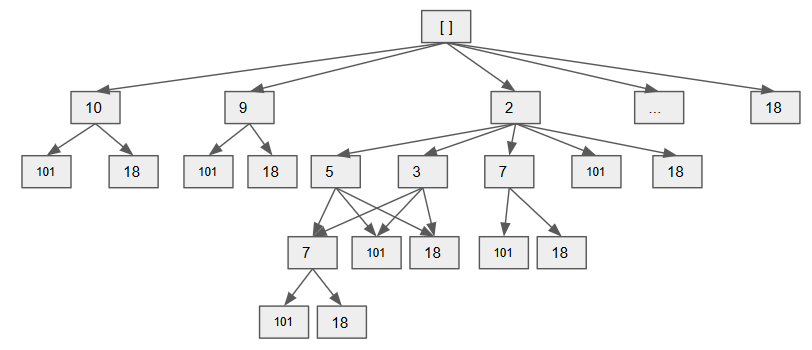
\includegraphics[width=\columnwidth]{fig/LIS_tree.png}
    \caption{State Transfer Tree Structure for LIS, each path represents a possible solution. Each arrow represents an move: find an element in the following elements that's larger than the current node.}
    \label{fig:tree_lis}
\end{figure}
\textbf{Solution 1: Induction}. For each subproblem, we show the result as follows. Each state dp[i] we represents the longest increasing subsequence ends with nums[i]. The reconstruction depends on all the previous i-1 subproblems, as shown in Eq.~\ref{LIS_equation_2}.
\begin{lstlisting}
subproblem: [], [10], [10,9], [10,9,2],[10,9,2,5],[10,9,2,5,3], [10,9,2,5,3, 7]...
Choice: 
ans:         0,  1,    1,       1,        2,          2,           3,         
\end{lstlisting}
\begin{equation}
\label{LIS_equation_2}
    f(i) = \begin{cases}
    1 + max(f(j)),& 0<j<i, arr[j] < arr[i];\\
    1& \text{otherwise}
    \end{cases}
\end{equation}
\begin{lstlisting}[language= Python]
class Solution(object):
    def lengthOfLIS(self, nums):
        """
        :type nums: List[int]
        :rtype: int
        """
        max_count = 0
        LIS = [0]*(len(nums)+1) # the LIS for array ends with index i
        for i in range(len(nums)): # start with 10
            max_before = 0
            for j in range(i): 
                if nums[i] > nums[j]:
                    max_before = max(max_before, LIS[j+1])
            LIS[i+1] = max_before+1
        return max(LIS)
\end{lstlisting}
\end{examples}

\subsection{Splitting}
Need to figure out how to fill out the two-dimensional dp matrix for splitting. 
\begin{examples}[resume]
\item \textbf{Word Break (L139, **).} Given a non-empty string s and a dictionary wordDict containing a list of non-empty words, determine if s can be segmented into a space-separated sequence of one or more dictionary words. \textit{Note: (1) The same word in the dictionary may be reused multiple times in the segmentation. (2) You may assume the dictionary does not contain duplicate words.}
\begin{lstlisting}[numbers=none]
Example 1:

Input: s = "leetcode", wordDict = ["leet", "code"]
Output: true
Explanation: Return true because "leetcode" can be segmented as "leet code".

Example 2:

Input: s = "applepenapple", wordDict = ["apple", "pen"]
Output: true
Explanation: Return true because "applepenapple" can be segmented as "apple pen apple".
             Note that you are allowed to reuse a dictionary word.

Example 3:

Input: s = "catsandog", wordDict = ["cats", "dog", "sand", "and", "cat"]
Output: false
\end{lstlisting}
\textbf{Solution: Induction + Splitting}. Like most of single sequence problem, we have n overlapping subproblems, for example of ``leetcode". 
\begin{lstlisting}[numbers=none]
subproblem: '', 'l', 'le', 'lee', 'leet', 'leetc', 'leetco', 'leetcod', 'leetcode'.
ans:         1,  0,    0,    0,     1,      0,       0,          0,         1
\end{lstlisting}
Thus, deduction still works here. We manually write down the result of each subproblem. Suppose we are trying to achieve answer for 'leet', how does it work?
if 'lee' is true and 't' is true, then we have true. Or, if 'le' is true, and 'et' is ture, we have true. unlike problems before, the ans for 'leet' can only be constructured from all the previous smaller problems. 
\begin{lstlisting}[language=Python]
def wordBreak(self, s, wordDict):
    wordDict = set(wordDict)
    n = len(s) 
    dp = [False]*(n+1)
    dp[0] = True #set 1 for empty str ''
    for i in range(1, n+1):
        for j in range(i):
            if dp[j] and s[j:i] in wordDict: # check previous result, and new word s[j:i]
                dp[i] = True

    return dp[-1]
\end{lstlisting}
\begin{figure}[h]
    \centering
    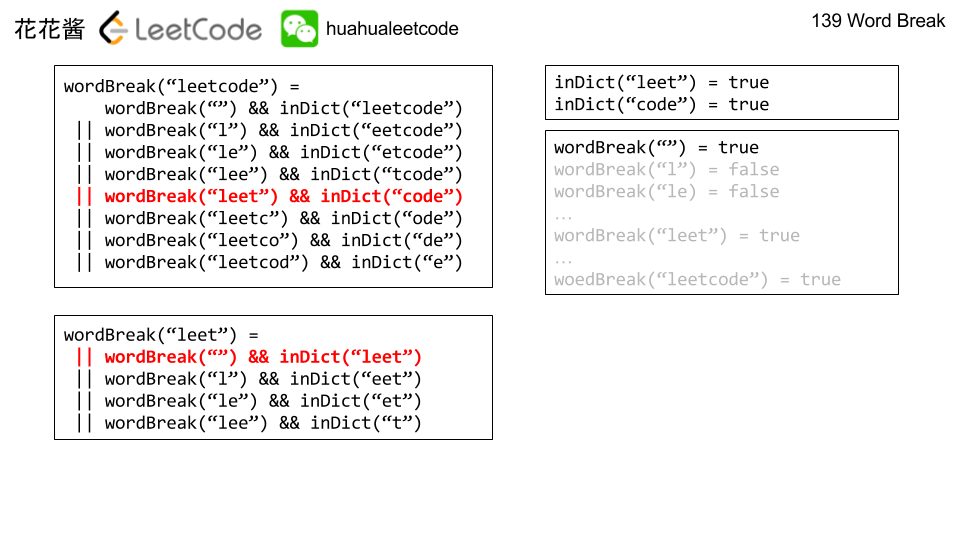
\includegraphics[width=0.8\columnwidth]{fig/word_break_139.png}
    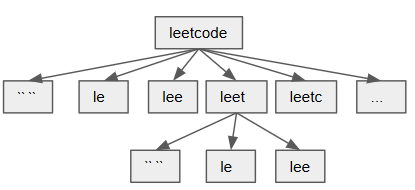
\includegraphics[width=0.8\columnwidth]{fig/tree_word_break.png}
    \caption{Word Break with DFS. For the tree, each arrow means check the word = parent-child and then recursively check the result of child. }
    \label{fig:word_break_dfs}
\end{figure}
\textbf{DFS+Memo}. To understand why each subproblem depends on $O(n)$ even smaller subproblem, we can look at the process solving the problem with DFS shown in Fig.~\ref{fig:word_break_dfs} (we can also draw a tree structure which will be more obvious). For ``leetcode" and ``leet" they both computed the subproblem '', 'l','le', 'lee'. Thus we can use memory to save solved problems. From the tree strcture, for each root node, it has $O(n)$ subbranches. So we should see why. To complete this, we give the code for the DFS version.
\begin{lstlisting}[language=Python]
def wordBreak(self, s, wordDict):
    wordDict = set(wordDict)
    #backtracking
    def DFS(start, end, memo):
        if start >= end:
            return True
        if start not in memo:
            if s[start:end] in wordDict:
                memo[start] = True
                return memo[start]
        
            for i in range(start, end+1):
                word = s[start:i] #i is the splitting point
                if word in wordDict:
                    if i not in memo:
                        memo[i] = DFS(i, end, memo)
                    if memo[i]:
                        return True
        memo[start] = False
                
        return memo[start]

    return DFS(0, n, {})
\end{lstlisting}
 \item \textbf{ Palindrome Partitioning II (L132, ***)} Given a string s, partition s such that every substring of the partition is a palindrome. Return the minimum cuts needed for a palindrome partitioning of s.
\begin{lstlisting}[numbers=none]
Example:

Input: "aab"
Output: 1
Explanation: The palindrome partitioning ["aa","b"] could be produced using 1 cut.
\end{lstlisting}
\textbf{Solution: use two dp.} one to track if it is pal and the other is to compute the cuts. 
\begin{lstlisting}[language = Python]
    def minCut(self, s):
        """
        :type s: str
        :rtype: int
        """
        pal = [[False for _ in range(len(s))] for _ in range(len(s))]
        cuts = [len(s)-i-1 for i in range(len(s))]
        for start in range(len(s)-1,-1,-1):
            for end in range(start, len(s)):
                if s[start] == s[end] and (end-start < 2 or pal[start+1][end-1]):
                    pal[start][end] = True
                    if end == len(s)-1:
                        cuts[start] = 0
                    else:
                        cuts[start] = min(cuts[start], 1+cuts[end+1])
        return cuts[0]
\end{lstlisting}
\item \textbf{Best Time to Buy and Sell Stock III (L123, hard).} Say you have an array for which the ith element is the price of a given stock on day i. Design an algorithm to find the maximum profit. You may complete at most two transactions. \textit{Note: You may not engage in multiple transactions at the same time (i.e., you must sell the stock before you buy again).}
\begin{lstlisting}[numbers=none]
Example 1:

Input: [3,3,5,0,0,3,1,4]
Output: 6
Explanation: Buy on day 4 (price = 0) and sell on day 6 (price = 3), profit = 3-0 = 3.
             Then buy on day 7 (price = 1) and sell on day 8 (price = 4), profit = 4-1 = 3.

Example 2:
\begin{lstlisting}
Input: [1,2,3,4,5]
Output: 4
Explanation: Buy on day 1 (price = 1) and sell on day 5 (price = 5), profit = 5-1 = 4.
             Note that you cannot buy on day 1, buy on day 2 and sell them later, as you are
             engaging multiple transactions at the same time. You must sell before buying again.

Example 3:
Input: [7,6,4,3,1]
Output: 0
Explanation: In this case, no transaction is done, i.e. max profit = 0.
\end{lstlisting}
\textbf{Solution:} the difference compared with I is that we need at most two times of transaction. We split the array into two parts from i, the max profit we can get till i and the max profit we can get from i to n. To get the maximum profit of each part is the same as the problem I. At last, the answer is max{preProfit[i] + postProfit[i]},$(0\leq i\leq n-1)$. However, we would get $O(n^2)$ time complexity if we use the following code, it has a lot of redundency. 
\begin{lstlisting}[language=Python]
from sys import maxsize
class Solution:
    def maxProfit(self, prices):
        """
        :type prices: List[int]
        :rtype: int
        """
        def maxProfitI(start, end):
            
            if start == end:
                return 0
            max_global_profit = 0
            min_local = prices[start]
            for i in range(start+1, end+1):
                max_global_profit= max(max_global_profit, prices[i]-min_local)
                min_local = min(min_local, prices[i])
            return max_global_profit
        
        if not prices:
            return 0
        n = len(prices)
        min_local = prices[0]
        preProfit, postProfit = [0]*n, [0]*n
    
        for i in range(n):
            preProfit[i] = maxProfitI(0,i)
            postProfit[i] = maxProfitI(i,n-1)
        maxProfit = max([pre+post for pre, post in zip(preProfit, postProfit)])
        return maxProfit
\end{lstlisting}
To avoid repeat work, we can use a for loop to get all the value of preProfit, and use another to get values for postProfit. For the postProfit, we need to traverse from the end to the start of the array in reverse direction, this way we track the local\_max and the profit is going to be local\_max - prices[i], and both keep a global max profit. The code is as follows:
\begin{lstlisting}[language = Python]
def maxProfit(self, prices):
    """
    :type prices: List[int]
    :rtype: int
    """        
    if not prices:
        return 0
    n = len(prices)

    preProfit, postProfit = [0]*n, [0]*n
    #get preProfit, from 0-n, track the mini_local, global_max
    min_local = prices[0]
    max_global_profit = 0
    for i in range(1,n):
        max_global_profit= max(max_global_profit, prices[i]-min_local)
        min_local = min(min_local, prices[i])
        preProfit[i] = max_global_profit
    #get  postProfit, from n-1 to 0, track the max_local, global_min
    max_local = prices[-1]
    max_global_profit = 0
    for i in range(n-1, -1, -1):
        max_global_profit= max(max_global_profit, max_local-prices[i])
        max_local =  max(max_local, prices[i])
        postProfit[i] = max_global_profit
    # iterate preProfit and postProfit to get the maximum profit
    maxProfit = max([pre+post for pre, post in zip(preProfit, postProfit)])
    return maxProfit
\end{lstlisting}

818. Race Car (hard)
\end{examples}

%%%%%%%%%%%%%%%%%%%range type %%%%%%%%%%%%%%%%%%%%%%%%%%%
\section{Single Sequence $O(n^3)$}
The difference of this type of singe sequence is that there are not only n subproblems for a sequence of size n, each subarray is A[0:i], i=[0, n]. There will be $n^2$ subproblems, each states as subarray $A[i:j], i \leq j$. Usually for this type, it shows such optimal substructure $dp[i][j] = f(dp[i][k], dp[k][j]), k \in [i, j]$. This would give us the $O(n^3)$ time complexity and $O(n^2)$ space complexity. The classical examples of this type of problem is matrix-multiplcation as explained in \textit{Introduction to Algorithms} and stone game. 
\label{sec_single_n3}
\subsection{Interval}
Problems include Stone Game, Burst Ballons, and Scramble String. The features of this type of dynamic programming is we try to get the min/max/count of a range of array; and the state transfer function updates through the range by from the big range to small rang.

\begin{examples}[resume]
\item \textbf{486. Predict the Winner (medium)}
Given an array of scores that are non-negative integers. Player 1 picks one of the numbers from either end of the array followed by the player 2 and then player 1 and so on. Each time a player picks a number, that number will not be available for the next player. This continues until all the scores have been chosen. The player with the maximum score wins.

Given an array of scores, predict whether player 1 is the winner. You can assume each player plays to maximize his score.
\begin{lstlisting}[numbers=none]
Example 1: Input: [1, 5, 2]. Output: False

Explanation: Initially, player 1 can choose between 1 and 2. 
If he chooses 2 (or 1), then player 2 can choose from 1 (or 2) and 5. If player 2 chooses 5, then player 1 will be left with 1 (or 2). So, final score of player 1 is 1 + 2 = 3, and player 2 is 5. Hence, player 1 will never be the winner and you need to return False.

Example 2: Input: [1, 5, 233, 7]. Output: True

Explanation: Player 1 first chooses 1. Then player 2 have to choose between 5 and 7. No matter which number player 2 choose, player 1 can choose 233. Finally, player 1 has more score (234) than player 2 (12), so you need to return True representing player1 can win.
\end{lstlisting}
Note:
\begin{enumerate}
    \item 1 <= length of the array <= 20.
    \item Any scores in the given array are non-negative integers and will not exceed 10,000,000.
    \item If the scores of both players are equal, then player 1 is still the winner.
    \end{enumerate}
Solution: At first, we can not use $f[i]$ to denote the state, because we can choose element from both the left and the right side, we  use $f[i][j]$ instead, which represents the maximum value we can get from $i$ to $j$ range. Second, when we deal with problem with potential accumulate value, we can use $sum[i][j]$ to represent the sum in the range $i-j$. Each player take actions to maximize their total points, f[i][j], it has two choice: left, right, which left f[i+1][j] and f[i][j-1] respectively for player two to choose. In order to gain the maximum scores in range [i,j] we need to optimize it by making sure f[i+1][j] and f[i][j-1] we choose the mimum value from. Therefore, we have state transfer function: $f[i][j] = sum[i][j] - min(f[i+1][j], f[i][j-1])$. Each subproblem relys on only two subproblems, which makes the total time complexity $O(n^2)$.  This is actually a game theory type. According to the function: if the range is $1$, when $i==j$, the value is $nums[i]$, which is the initialization. For the loop, the first for loop is the range: from size $2$ to $n$, the second for loop to get the start index $i$ in range $[0, n-l]$, then the end index $j = i+l-1$. The answer for this problem is: if $f[0][-1]>=sum/2$. If it is, then it is true.

The process of the for loop is we initialize the diagonal element, and fill out element on the right upper side, which is upper diagonal. 
\begin{figure}[h]
    \centering
    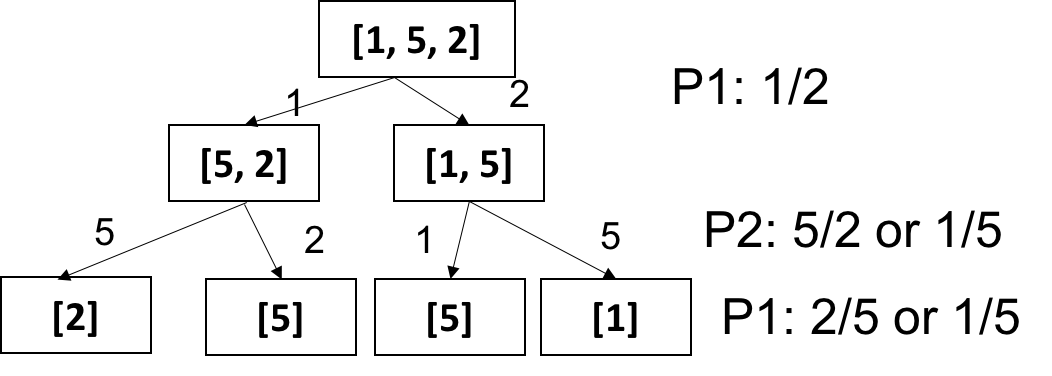
\includegraphics[width = 0.6\columnwidth]{fig/guesswinner.png}
    \caption{Caption}
    \label{fig:my_label}
\end{figure}
\begin{lstlisting}[language = Python]
def PredictTheWinner(nums):
        """
        :type nums: List[int]
        :rtype: bool
        """
        if not nums:
            return False
        if len(nums)==1:
            return True
        #sum[i,j] = sum[j+1]-sum[i]
        sums = nums[:]
        for i in range(1,len(nums)):
            sums[i]+=sums[i-1]
        sums.insert(0,0)
        
        dp=[[0 for col in range(len(nums))] for row in range(len(nums))]
        for i in range(len(nums)):
            dp[i][i] = nums[i]
        
        for l in range(2, len(nums)+1):
            for i in range(0,len(nums)-l+1): #start 0, end len -l+1
                j =i+l-1
                dp[i][j] = (sums[j+1]-sums[i])-min(dp[i+1][j],dp[i][j-1])
        n =len(nums)
        return dp[0][n-1]>=sums[-1]/2
\end{lstlisting}
Else, we use $f[i][j] = max(nums[i]-f[i+1][j], nums[j]-f[i][j-1])$ to represent the difference of the points gained by player one compared with player two. When $f[i][j]$ is the state of player one, then $f[i][j-1]$ and $f[i+1][j]$ are the potential states of player two. 
\begin{lstlisting}[language = Python]
class Solution:
    def PredictTheWinner(self, nums):
        """
        :type nums: List[int]
        :rtype: bool
        """
        n = len(nums)
        if n == 1 or n%2==0 : return True
        dp = [[0] * n for _ in range(n)]
        for l in range(2, len(nums)+1):
            for i in range(0,len(nums)-l+1): #start 0, end len -l+1
                j =i+l-1
                dp[i][j] = max(nums[j] - dp[i][j-1],nums[i] - dp[i+1][j])
        return dp[0][-1]>=0
\end{lstlisting}
Actually the for loop we can use a simpler one. However, it is harder to understand to code compared with the standard version.
\begin{lstlisting}[language = Python]
for i in range(n-1,-1,-1):
            dp[i][i] = nums[i] #initialization
            for j in range(i+1,n):
                dp[i][j] = max(nums[j] - dp[i][j-1],nums[i] - dp[i+1][j])
\end{lstlisting}


\item \textbf{Stone Game}

There is a stone game. At the beginning of the game the player picks n piles of stones in a line. The goal is to merge the stones in one pile observing the following rules:

 At each step of the game,the player can merge two adjacent piles to a new pile. The score is the number of stones in the new pile. You are to determine the minimum of the total score.
 Example
 For [4, 1, 1, 4], in the best solution, the total score is 18:

    Merge second and third piles [4, 2, 4], score $+2$
    Merge the first two piles [6, 4], score $+6$
    Merge the last two piles [10], score $+10$

Other two examples:
 [1, 1, 1, 1] return 8
 [4, 4, 5, 9] return 43

\item \textbf{312. Burst Balloons}

Given n balloons, indexed from 0 to n-1. Each balloon is painted with a number on it represented by array nums. You are asked to burst all the balloons. If the you burst balloon i you will get nums[left] * nums[i] * nums[right] coins. Here left and right are adjacent indices of i. After the burst, the left and right then becomes adjacent.

Find the maximum coins you can collect by bursting the balloons wisely.

Note: 
 (1) You may imagine nums[-1] = nums[n] = 1. They are not real therefore you can not burst them.
 (2) 0 $\leq$ nums[i] $\leq$  500, 0 $\leq$  nums[i] $\leq$  100
\begin{lstlisting}[numbers=none]
Example:

Given [3, 1, 5, 8]

Return 167

nums = [3,1,5,8] --> [3,5,8] -->   [3,8]   -->  [8]  --> []
   coins =  3*1*5      +  3*5*8    +  1*3*8      + 1*8*1   = 167
\end{lstlisting}

at first burst c[i][k-1] then burst c[k+1][j], then burst k,
\begin{lstlisting}[language = Python]
class Solution:
    def maxCoins(self, nums):
        """
        :type nums: List[int]
        :rtype: int
        """
        n = len(nums)
        nums.insert(0,1)
        nums.append(1)
        
        c = [[0 for _ in range(n+2)] for _ in range(n+2)]
        for l in range(1, n+1): #length [1,n]
            for i in range(1,n-l+2): #start [1, n-l+1]
                j = i+l-1 #end =i+l-1
                
                #function is a k for loop
                for k in range(i,j+1):
                    c[i][j] = max(c[i][j], c[i][k-1]+nums[i-1]*nums[k]*nums[j+1]+c[k+1][j])
        #return from 1 to n
        return c[1][n]
\end{lstlisting}

\item \textbf{516. Longest Palindromic Subsequence}

Given a string s, find the longest palindromic subsequence’s length in s. You may assume that the maximum length of s is 1000.
\begin{lstlisting}[numbers=none]
Example 1:

 Input:
"bbbab"
Output:
4
One possible longest palindromic subsequence is "bbbb".

Example 2:
 Input:
"cbbd"
Output:
2
One possible longest palindromic subsequence is "bb".
\end{lstlisting}

Solution: for this problem, we have state dp[i][j] means from i to j, the length of the longest palindromic subsequence. dp[i][i] = 1. Then we use this range to fill in the dp matrix (upper triangle.)
\begin{lstlisting}[language = Python]
def longestPalindromeSubseq(self, s):
        """
        :type s: str
        :rtype: int
        """
        nums=s
        if not nums:
            return 0
        if len(nums)==1:
            return 1
        
        def isPanlidrome(s):
            l,r= 0, len(s)-1
            while l<=r:
                if s[l]!=s[r]:
                    return False
                else:
                    l+=1
                    r-=1
            return True
        
        if isPanlidrome(s): #to speed up
            return len(s)
        
        rows=len(nums)
        dp=[[0 for col in range(rows)] for row in range(rows)]
        for i in range(0,rows):
            dp[i][i] = 1
        
        for l in range(2, rows+1): #use a length
            for i in range(0,rows-l+1): #start 0, end len -l+1
                j =i+l-1
                if j>rows:
                    continue
                if s[i]==s[j]:
                    dp[i][j] = dp[i+1][j-1]+2
                else:
                    left_size,right_size = dp[i][j-1],dp[i+1][j]
                    dp[i][j]= max(dp[i][j-1], right_size)
        print(dp)
        return dp[0][rows-1]
\end{lstlisting}

Or else, we can say, i need to be from i+1 to i, from big to small, j need to from j-1 or j to j, from small to big.
\begin{lstlisting}[language = Python]
for (int i = n - 1; i >= 0; --i) {
            dp[i][i] = 1;
            for (int j = i + 1; j < n; ++j) {
                if (s[i] == s[j]) {
                    dp[i][j] = dp[i + 1][j - 1] + 2;
                } else {
                    dp[i][j] = max(dp[i + 1][j], dp[i][j - 1]);
                }
            }
        }
\end{lstlisting}

Now to do the space optimization:
\begin{lstlisting}[language = Python]
class Solution {
public:
    int longestPalindromeSubseq(string s) {
        int n = s.size(), res = 0;
        vector<int> dp(n, 1);
        for (int i = n - 1; i >= 0; --i) {
            int len = 0;
            for (int j = i + 1; j < n; ++j) {
                int t = dp[j];
                if (s[i] == s[j]) {
                    dp[j] = len + 2;
                } 
                len = max(len, t);
            }
        }
        for (int num : dp) res = max(res, num);
        return res;
    }
};
\end{lstlisting}
\end{examples}
    %%%%%%%%%%%%%%%%%%%Coordinate: BFS and DP %%%%%%%%%%%%%%%%%%%%%%%%%%%
\section{Coordinate: BFS and DP}
\label{sec_coordinate}
In this type of problems, we are give an array or a matrix with $1$D or $2$D axis. We either do 'optimization' to find the minimum path sum, or do the 'counting' to get the total number of paths, or check if we can start from A and end at B. %The four key elements for type of dynamic programming: 

\textbf{Two-dimensional}. For a $O(mn)$ sized coordinate, Tab.~\ref{tab:2d_coordinate} shows two different types: one there will only be $O(mn)$, and the other is $O(kmn)$, $k$ here normally represents number of steps. Because a 2D coordinate is inherently a graph, so this type is closely related to the graph traversal algorithms; BFS for counting and DFS for the optimization problems. 
\begin{table}[h]
\begin{small}
\centering
\noindent\captionof{table}{ Different Type of Coordinate Dynamic Programming}
 \noindent \begin{tabular}{|p{0.14\columnwidth}|p{0.14\columnwidth}| p{0.14\columnwidth}|p{0.14\columnwidth}|p{0.14\columnwidth}|p{0.14\columnwidth}|}
  \hline
 Case & Input & Subproblems & f(n) & Time & Space   \\ \hline
Easy  & $O(mn)$& $O(mn)$ & $O(1)$ & $O(mn)$ & $O(mn)->O(m)$ \\\hline
Medium  & $O(mn)$& $O(kmn)$ & $O(1)$ & $O(kmn)$ & $O(kmn)->O(mn)$\\ \hline
\end{tabular}
  \label{tab:2d_coordinate}
  \end{small}
\end{table}
% \begin{enumerate}
For this type of problems, understanding the BFS related solution is more important than just mesmorizing the template of the dynamic programming solution. There, we will use two sections: Counting: BFS and DP in Sec.~\ref{sec_coordinate_counting} and Optimization in Sec.~\ref{} with LeetCode examples to learn how to solve this type of dynamic programming problems. 
% \item state $f[x]$ denotes state from the starting point to axis $x$, for $2$D, we use $f[x][y]$ denotes the state from $x$ to $y$; Will have $n$ or $m\times n$ space. 
% \item function: we need to find the relation between $f[x]$ or $f[x][y]$ with its previous state (from top-down) or afterwards state.
% \item initialization: initialze the first column and first row, and sometimes is the first column and the last column. Initialize the edge condition that can not compleete the function. 
% \item answer: $f[n-1]$ or $max(f)$ or $f[-1][-1]$
% \end{enumerate}

%%%%%%%%%%%%%%%%%%%One Time Traversal %%%%%%%%%%%%%%%%%%%%%%%%%%%
\subsection{One Time Traversal}
\label{sec_coordinate_counting}
In this section, we want to explore how we can modify our solution from BFS to the dynamic programming. Inherently, dynamic programming solutions for this type of problems are the optimized Breath-first-search. 

\subsubsection{Counting} In this type, any location in the coordinate will be only vised once. Thus, it gives $O(mn)$ time complexity. 

62. Unique Paths
\begin{lstlisting}
A robot is located at the top-left corner of a m x n grid (marked 'Start' in the diagram below).

The robot can only move either down or right at any point in time. The robot is trying to reach the bottom-right corner of the grid (marked 'Finish' in the diagram below).

How many possible unique paths are there?

Above is a 3 x 7 grid. How many possible unique paths are there?

Note: m and n will be at most 100.

Example 1:

Input: m = 3, n = 2
Output: 3
Explanation:
From the top-left corner, there are a total of 3 ways to reach the bottom-right corner:
1. Right -> Right -> Down
2. Right -> Down -> Right
3. Down -> Right -> Right

Example 2:

Input: m = 7, n = 3
Output: 28
\end{lstlisting}
\begin{figure}[h]
    \centering
    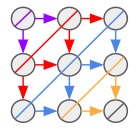
\includegraphics[width=0.6\columnwidth]{fig/unique_path.png}
    \caption{One Time Graph Traversal. Different color means different levels of traversal.}
    \label{fig:unique_path}
\end{figure}
\textbf{BFS}. Fig.~\ref{fig:unique_path} shows the BFS traversal process in the matrix. We can clearly see that each node and edge is only visited once. The BFS solution is straightforward and is the best solution. We use bfs to track the nodes in the queue at each level, and dp to record the unique paths to location $(i,j)$. Because each location is only visted once, thus, at each level, using the same dp will have no conflict.  
\begin{lstlisting}[language = Python]
# BFS
def uniquePaths(self, m, n):
    dp = [[0 for _ in range(n)] for _ in range(m)]
    dp[0][0] = 1
    bfs = set([(0,0)])
    dirs = [(1, 0), (0,1)]
    while bfs:
        new_bfs = set()
        for x, y in bfs:
            for dx, dy in dirs:
                nx, ny = x+dx, y+dy
                if 0<=nx<m and 0<=ny<n:
                    dp[nx][ny]+= dp[x][y]
                    new_bfs.add((nx, ny))
        bfs = new_bfs
    return dp[m-1][n-1]
\end{lstlisting}

\textbf{Dynamic Programming}. In the BFS solution, we use a set to track  the nodes at each level. However, its corresponding dynamic programming solution should design a way to obtain the result of current state only dependent on the previous computed state. Here each position has a different state:  $(x, y)$ and $f[x][y]$ denotes the number of unique paths from start position (0, 0) to $(x, y)$. The state transfer function: $f[x][y] = f[x-1][y] + f[x][y -1]$. If we initialize the boundary locations (the first row and the first column), and we visit each location by loop over row and col, then we can get the dynamic programming solution. 

\begin{lstlisting}[language = Python]
def uniquePaths(self, m, n):
        if m==0 or n==0:
            return 0
        dp =[[0 for col in range(n)] for row in range(m)]
        dp[0][0]=1
        #initialize row 0
        for col in range(1,n):
            dp[0][col] = dp[0][col-1]
        #initialize col 0
        for row in range(1,m):
            dp[row][0] = dp[row-1][0]
        
        for row in range(1,m):
            for col in range(1,n):
                dp[row][col]=dp[row-1][col]+dp[row][col-1]
        return dp[m-1][n-1]
\end{lstlisting}
377. Combination Sum IV (medium)
\begin{lstlisting}
 Given an integer array with all positive numbers and no duplicates, find the number of possible combinations that add up to a positive integer target.

Example:

nums = [1, 2, 3]
target = 4

The possible combination ways are:
(1, 1, 1, 1)
(1, 1, 2)
(1, 2, 1)
(1, 3)
(2, 1, 1)
(2, 2)
(3, 1)

Note that different sequences are counted as different combinations.

Therefore the output is 7.

Follow up:
What if negative numbers are allowed in the given array?
How does it change the problem?
What limitation we need to add to the question to allow negative numbers? 
\end{lstlisting}
\textbf{Target as Climbing Stairs}. Analysis: The DFS+MEMO solution is given in Section~\ref{sec_combination}. However, because we just need to count the number, which makes the dynamic programming possible. From the DFS solution, we can see the state depends on the target, thus we can define a dp array that use (target+1) space. This is like climbing stairs, each time we can either go 1, or 2, or 3 steps. 
\begin{lstlisting}
[1,2,3], t = 4
t = 0: dp[0] = 1, []
t = 1: t(0)+1, dp[1] = 1; [1]
t = 2: t(0)+2, dp[2] = 1,t(1)+1, dp[2]+=1, dp[2] = 2; [2], [1, 1]
t = 3: t(0)+3, dp[3]=1, t(1)+2, dp[3]+=1, t(2)+1, dp[3]+=2, dp[3] = 4, [3],[1,2],[2,1],[1,1,1]
t = 4: t(0)+4, dp[4]=0, t(1)+3, dp[4]+=1, t(2)+2, dp[4]+=2, t(3)+1, dp[4]+=4, dp[4] = 7, [1, 3], [2,2], [1, 1, 2], [3, 1], [1,2,1],[2,1,1], [1,1,1,1]
\end{lstlisting}
\begin{lstlisting}[language=Python]
def combinationSum4(self, nums, target):
    """
    :type nums: List[int]
    :type target: int
    :rtype: int
    """
    nums.sort()
    n = len(nums)
    dp = [0]*(target+1)
    dp[0] = 1
    for t in range(1, target+1):
        for n in nums:
            if t-n >= 0:
                dp[t] += dp[t-n]
            else:
                break
    return dp[-1]
\end{lstlisting}
\subsubsection{Optimization}
64. Minimum Path Sum (medium)
\begin{lstlisting}

Given a m x n grid filled with non-negative numbers, find a path from top left to bottom right which minimizes the sum of all numbers along its path.

Note: You can only move either down or right at any point in time.

Example 1:

[[1,3,1],
 [1,5,1],
 [4,2,1]]
\end{lstlisting}

Given the above grid map, return 7. Because the path $1\rightarrow3\rightarrow1\rightarrow1\rightarrow1$ minimizes the sum.
\begin{figure}[h]
    \centering
    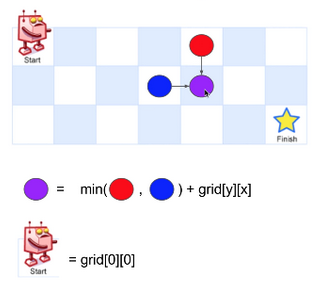
\includegraphics[width = 0.5\columnwidth] {fig/min_path.png}
    \caption{Caption}
    \label{fig:my_label}
\end{figure}
\textbf{Dynamic Programming}. For this problem, it is exactly the same as all the previous problems, the only difference is the state transfer function. $f(i,j) = g(i,j) + min(f(i-1, j), f(i, j-1))$. 
\begin{lstlisting}[language = Python]
# dynamic programming
def minPathSum(self, grid):
    if not grid:
        return 0
    rows, cols = len(grid), len(grid[0])
    dp = [[0 for _ in range(cols)] for _ in range(rows)]
    dp[0][0] = grid[0][0]
    
    # initialize row
    for c in range(1, cols):
        dp[0][c] = dp[0][c-1] + grid[0][c]
    
    # initialize col
    for r in range(1, rows):
        dp[r][0] = dp[r-1][0] + grid[r][0]
        
    for r in range(1, rows):
        for c in range(1, cols):
            dp[r][c] = grid[r][c] + min(dp[r-1][c], dp[r][c-1])
    return dp[-1][-1]
\end{lstlisting}
\textbf{Dynamic Programming with Space Optimization}. As can be seen, each time when we update $sum[i][j]$, we only need $sum[i - 1][j]$ (at the current column) and $sum[i][j - 1]$ (at the left column). So we need not maintain the full $m*n$ matrix. Maintaining two columns is enough and now we have the following code.
\begin{lstlisting}[language = Python]
rows, cols= len(grid),len(grid[0])
        #O(rows) 
        pre, cur =[0]*rows, [0]*rows
        #intialize the the first col, walk from the (0,0)->(1,0)->(row,0)
        pre[0]=grid[0][0]

        for row in range(1, rows):
            pre[row]=pre[row-1]+grid[row][0] #this is equal to cost[0][row]
        for col in range(1, cols):
            cur[0] = pre[0]+grid[0][col]  #initialize the first row, current [0][0]
            for row in range(1, rows):
                cur[row]= min(cur[row-1], pre[row])+grid[row][col]
            pre,cur = cur, pre
        return pre[rows-1]
\end{lstlisting}

Further inspecting the above code, it can be seen that maintaining pre is for recovering $pre[i]$, which is simply $cur[i]$ before its update. So it is enough to use only one vector. Now the space is further optimized and the code also gets shorter.
\begin{lstlisting}[language = Python]
rows, cols= len(grid),len(grid[0])
        #O(rows) 
        cur = [0]*rows
        #intialize the the first col, walk from the (0,0)->(1,0)->(row,0)
        cur[0]=grid[0][0]
        for row in range(1, rows):
            cur[row]=cur[row-1]+grid[row][0]
        for col in range(1, cols):
            cur[0] = cur[0]+grid[0][col]  #initialize the first row
            for row in range(1, rows):
                cur[row]= min(cur[row-1], cur[row])+grid[row][col]
        return cur[rows-1]
\end{lstlisting}

Now, we use O(1) space by reusing the original grid.
\begin{lstlisting}[language = Python]
rows, cols= len(grid),len(grid[0])
        #O(1) space by reusing the space here
        for i in range(0, rows):
            for j in range(0, cols):
                if i==0 and j ==0:
                    continue
                elif i==0 :
                    grid[i][j]+=grid[i][j-1]
                elif j==0:
                    grid[i][j]+=grid[i-1][j]
                else:
                    grid[i][j]+= min(grid[i-1][j], grid[i][j-1])
        return grid[rows-1][cols-1]
\end{lstlisting}
%%%%%%%%%%%%%%%%%%%Multiple-time Traversal %%%%%%%%%%%%%%%%%%%%%%%%%%%
\subsection{Multiple-time Traversal}
In this type, we need to traverse each location for K times, making K steps of moves thus we can get the final solution. This will have $O(kmn)$ time complexity. 
\subsubsection{Two-dimensional Coordinate}
935. Knight Dialer (Medium)
\begin{figure}
    \centering
    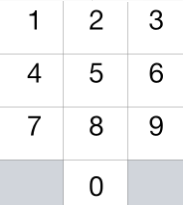
\includegraphics{fig/knight_dialer.png}
    \caption{Caption}
    \label{fig:my_label}
\end{figure}
\begin{lstlisting}
A chess knight can move as indicated in the chess diagram below:
This time, we place our chess knight on any numbered key of a phone pad (indicated above), and the knight makes N-1 hops.  Each hop must be from one key to another numbered key.

Each time it lands on a key (including the initial placement of the knight), it presses the number of that key, pressing N digits total.

How many distinct numbers can you dial in this manner?

Since the answer may be large, output the answer modulo 10^9 + 7.

Example 1:

Input: 1
Output: 10

Example 2:

Input: 2
Output: 20

Example 3:

Input: 3
Output: 46

Note:

    1 <= N <= 5000
\end{lstlisting}
\textbf{Most Naive BFS}. Analysis: First, we need to figure out from each number, where is the possible next moves.  We would have get this dictionary: $moves = \{0:[4, 6], 1:[6, 8], 2: [7, 9], 3: [4,8], 4: [0, 3, 9], 5:[], 6:[0,1,7], 7:[2,6], 8:[1,3],9:[2,4]\}$. This is not exactly a coordinate, however, because we can make endless move, we would have a graph. The brute force is we put [0,1,2,3,4,5,6,7,8,9] as the start positions, and we use BFS to control the steps, the total number of paths is the sum over of all the leaves. At each step, we would do two things 1) generate a list to save all the possible next numbers; 2) if it reaches to the leaves, sum up all the nodes. 
\begin{lstlisting}[language = Python]
# naive BFS solution
def knightDialer(self, N):
    """
    :type N: int
    :rtype: int
    """
    if N == 1:
        return 10
    moves = {0:[4, 6], 1:[6, 8], 2: [7, 9], 3: [4,8], 4: [0, 3, 9], 5:[], 6:[0,1,7], 7:[2,6], 8:[1,3],9:[2,4]} #4, 6 has three

    bfs = [0, 1, 2, 3, 4, 5, 6, 7, 8, 9] # all starting points
    step = 1
    while bfs:
        new = []
        for i in bfs: 
            new += moves[i]
        step += 1
        bfs = new
        if step == N:
            return len(bfs)%(10**9+7)
\end{lstlisting}
\textbf{Optimized BFS}. However, the brute force BFS only passed 18/120 test cases. To improve it further, we know that we only need a counter to record the counter of each number in that level. This way, bfs is replaced with a counter. Now, the new code is:
\begin{lstlisting}[language = Python]
#optimized BFS exactly a DP
def knightDialer(self, N):
    MOD = 10**9+7
    if N == 1:
        return 10
    moves = {0:[4, 6], 1:[6, 8], 2: [7, 9], 3: [4,8], 4: [0, 3, 9], 5:[], 6:[0,1,7], 7:[2,6], 8:[1,3],9:[2,4]} #4, 6 has three

    bfs = [1]*10
    step = 1

    while bfs:
        size = 0
        new = [0]*10
        for idx, count in enumerate(bfs): 
            for m in moves[idx]:
                new[m] += count
                new[m] %= MOD
        step += 1
        bfs = new
        if step == N:
            return sum(bfs)%(MOD)
\end{lstlisting}
\textbf{Optimized Dynamic Programming}. This is exactly a dynamic programming algorithm: $new[m] += bfs[i]$, for example, from 1 we can move to 6,8,so that we have $f(1,n) = f(6, n-1) + f(8, n-1)$. So here a state is represented by $bfs[num]$ and $step$, and it saves the count at each state. Now, we write it in the way of dp template:
\begin{lstlisting}[language=Python]
# optimized dynamic programming template
def knightDialer(self, N):
    MOD = 10**9+7
    moves = {0:[4, 6], 1:[6, 8], 2: [7, 9], 3: [4,8], 4: [0, 3, 9], 5:[], 6:[0,1,7], 7:[2,6], 8:[1,3],9:[2,4]} #4, 6 has three

    dp = [1]*10
    
    for step in range(N-1):
        size = 0
        new_dp = [0]*10
        for idx, count in enumerate(dp): 
            for m in moves[idx]:
                new_dp[m] += count
                new_dp[m] %= MOD
        dp = new_dp
   
    return sum(dp)%(MOD)
\end{lstlisting}
% \begin{lstlisting}[language = Python]
% # optimized BFS
% def knightDialer(self, N):
%     """
%     :type N: int
%     :rtype: int
%     """
%     if N == 1:
%         return 10
%     moves = {0:[4, 6], 1:[6, 8], 2: [7, 9], 3: [4,8], 4: [0, 3, 9], 5:[], 6:[0,1,7], 7:[2,6], 8:[1,3],9:[2,4]} #4, 6 has three

%     bfs = collections.Counter([0, 1, 2, 3, 4, 5, 6, 7, 8, 9])
%     step = 1

%     while bfs:
%         size = 0
%         new = collections.Counter()
%         for i in bfs: 
%             for m in moves[i]:
%                 new[m] += bfs[i]
%         step += 1
%         bfs = new
%         if step == N:
%             return sum(bfs.values())%(10**9+7)
% \end{lstlisting}
%Now, this updated algorithm passed 93/120 test cases. 



688. Knight Probability in Chessboard (Medium)
\begin{lstlisting}
On an NxN chessboard, a knight starts at the r-th row and c-th column and attempts to make exactly K moves. The rows and columns are 0 indexed, so the top-left square is (0, 0), and the bottom-right square is (N-1, N-1).

A chess knight has 8 possible moves it can make, as illustrated below. Each move is two squares in a cardinal direction, then one square in an orthogonal direction.

Each time the knight is to move, it chooses one of eight possible moves uniformly at random (even if the piece would go off the chessboard) and moves there.

The knight continues moving until it has made exactly K moves or has moved off the chessboard. Return the probability that the knight remains on the board after it has stopped moving.

Example:

Input: 3, 2, 0, 0
Output: 0.0625
Explanation: There are two moves (to (1,2), (2,1)) that will keep the knight on the board.
From each of those positions, there are also two moves that will keep the knight on the board.
The total probability the knight stays on the board is 0.0625.
\end{lstlisting}
\textbf{Optimized BFS}. Analysis: Each time we can make 8 moves, thus after K steps, we can have $8^K$ total unique paths. Thus, we just need to get the total number of paths that it ends within the board (valid paths). The first step is to write down the possible moves or directions. And, then we initialize a two-dimensional array $dp$ to record the number of paths end at $(i, j)$ after $k$ steps. Using a BFS solution, each time we just need to save all the unique positions can be reached at that step. 
\begin{lstlisting}[language=Python]
# Optimized BFS solution
def knightProbability(self, N, K, r, c):
    dirs = [[-2, -1], [-2, 1], [-1, -2], [-1, 2], [1, -2], [1, 2], [2,-1],[2, 1]]
    dp = [[0 for _ in range(N)] for _ in range(N) ]
    total = 8**K
    last_pos = set([(r, c)])
    dp[r][c]=1

    for step in range(K):
        new_pos = set()
        new_dp = [[0 for _ in range(N)] for _ in range(N) ]
        for x, y in last_pos:
            for dx, dy in dirs:
                nx = x+dx
                ny = y+dy
                if 0<=nx<N and 0<=ny<N:
                    new_dp[nx][ny] += dp[x][y]
                    new_pos.add((nx, ny))
        last_pos = new_pos
        dp = new_dp

    return float(sum(map(sum, dp)))/total
\end{lstlisting}
\textbf{Optimized Dynamic Programming}. If we delete the last\_pos and directly use the dp to use as a way to visit the last positions, this is a space optimized dynamic programming solution. And this solution is nearly the fastest; compared with the above solution, each step we cut down the cost of maintain a set (a hashmap) dynamically. 
\begin{lstlisting}[language = Python]
# Best Dynamic Programming Solution
def knightProbability(self, N, K, r, c):
    dirs = [[-2, -1], [-2, 1], [-1, -2], [-1, 2], [1, -2], [1, 2], [2,-1],[2, 1]]
    dp = [[0 for _ in range(N)] for _ in range(N) ]
    total = 8**K
    dp[r][c]=1

    for step in range(K):
        new_dp = [[0 for _ in range(N)] for _ in range(N) ]
        for i in range(N):
            for j in range(N):
                if dp[i][j] == 0:
                    continue #not available position
                for dx, dy in dirs:
                    nx, ny = i+dx, j+dy
                    if 0<=nx<N and 0<=ny<N:
                        new_dp[nx][ny] += dp[i][j]
        dp = new_dp

    return float(sum(map(sum, dp)))/total
\end{lstlisting}

\subsubsection{One-dimensional Coordinate}
For one-dimensional, it is the same as two-dimensional, and it could be even simpler. 

70. Climbing Stairs (Easy)
\begin{lstlisting}
You are climbing a stair case. It takes n steps to reach to the top.

Each time you can either climb 1 or 2 steps. In how many distinct ways can you climb to the top?

Note: Given n will be a positive integer.

Example 1:

Input: 2
Output: 2
Explanation: There are two ways to climb to the top.
1. 1 step + 1 step
2. 2 steps

Example 2:

Input: 3
Output: 3
Explanation: There are three ways to climb to the top.
1. 1 step + 1 step + 1 step
2. 1 step + 2 steps
3. 2 steps + 1 step
\end{lstlisting}
\begin{figure}[h]
    \centering
    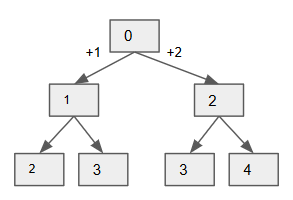
\includegraphics[width=0.6\columnwidth]{fig/climbing_stair.png}
    \caption{Tree Structure for One dimensional coordinate}
    \label{fig:tree_climbing_stair}
\end{figure}
\textbf{BFS}. Fig~\ref{fig:tree_climbing_stair} demonstrates the state transfer relation between different position. First, we can solve it using our standard BFS. In this problem, we do not know the level of the tree structure, so the end condition is while the bfs is not empty. Thus, eventually the bfs is set to empty, and the result of the dp is empty too. So we use a global variable $ans$ to track our result.
\begin{lstlisting}[language=Python]
# BFS
def climbStairs(self, n):
    dp = [0]*(n+1)
    dp[0] = 1 # init starting point 0 to 1
    dirs = [1, 2]
    bfs = set([0])
    ans = 0
    while bfs:
        new_dp = [0]*(n+1)
        new_bfs = set()
        for i in bfs: #pos 
            for dx in dirs:
                nx = i+dx
                if 0 <= nx <= n:
                    new_dp[nx] += dp[i]
                    new_bfs.add(nx)
        ans += dp[-1]
        bfs, dp = new_bfs, new_dp
    return ans
\end{lstlisting}
\textbf{Dynamic Programming}. If we observe the tree structure, we have the state transfer function $f(i) = f(i-1) + f(i-2)$. Thus, a single for loop starts from 2, the dp list can be filled in without overlap. 
\begin{lstlisting}[language=Python]
# Dynamic Programming
def climbStairs(self, n):
    dp = [0]*(n+1)
    dp[0] = 1 # init starting point 0 to 1
    dp[1] = 1
    
    for i in range(2, n+1):
        dp[i] = dp[i-1] + dp[i-2]
    return dp[-1]
\end{lstlisting}
The BFS and the Dynamic Programming has the same time and space complexity.

%%%%%%%%%%%%%%%%%%%Generalize %%%%%%%%%%%%%%%%%%%%%%%%%%%
\subsection{Generalization}
\begin{enumerate}
    \item State: $f[x]$ or $f[x][y]$ to denote the optimum value or count, or check the workability of whole solutions till axis $x$ for $1$D and $(x,y)$ for $2$D;  
    \item Function: usually for $f[x]$, we connect $f[x]R f[x-1]$, or $f[x][y] R f[x-1][y], f[x][y-1]$;   
    \item Initialization: for $f[x]$ we initialize the starting point, sometimes we need extra $1$ space, with size $n+1$;  for $f[x][y]$ we need to initialize elements from row $0$ and col $0$;
    \item Answer: Usually it is $f[n-1]$ or $f[m-1][n-1]$; 
\end{enumerate}
\textbf{Space Optimization} For $f[i] = max(f[i-1], f[i-2] + A[i])$, it can be converted into $f[i\%2] = max(f[(i-1)\%2], f[(i-2)\%2])$. Also, we can directly using the original matrix or array to save the state results.  Note: there are possible ways to optimize the space complexity, we can do it from $O(m*n)$ to $O(m+n)$ to $O(1)$ which we get by reusing the original grid or array.
\subsubsection{One-Time Traversal}
\begin{lstlisting}
dp[i][j] := answer of A[0->i][0->j]

#template
dp[n+1][m+1]
for i in range(n):
    for j in range(m):
        dp[i][j] = f(dp[pre_i][pre_j])
return f(dp)
\end{lstlisting}

\subsubsection{Multiple-Dimensional Traversal}
\begin{lstlisting}
dp[k][i][j] := answer of A[0->i][0->j] after k steps

#template
dp[k][n+1][m+1]
for _ in range(k):
    for i in range(n):
        for j in range(m):
            dp[k][i][j] = f(dp[k-1][pre_i][pre_j])
return f(dp)
\end{lstlisting}




%%%%%%%%%%%%%%%%%%%double sequence %%%%%%%%%%%%%%%%%%%%%%%%%%%
\section{Double Sequence: Pattern Matching DP}
\label{sec_double_sequence}
\begin{figure}[h!]
    \centering
    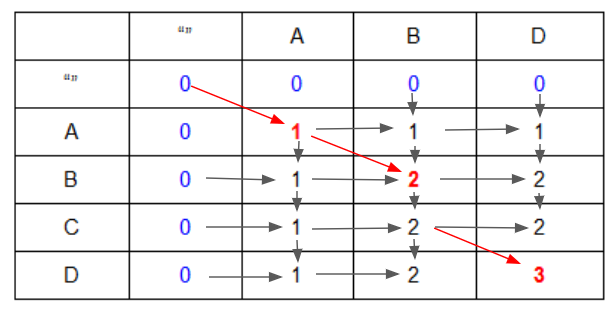
\includegraphics[width=0.7\columnwidth]{fig/lcs_problem.png}
    \caption{Longest Common Subsequence}
    \label{fig:lcs}
\end{figure}
In this section, we focus on double sequence P and S with input size $O(m)+O(n)$. Because double sequence can naturally be arranged to be a matrix with size $(m+1)\times(n+1)$. Here we have extra row and extra column, it happens because we put empty char '' at the beginning of each string to better initialize and get result even for empty string too. One example is shown in Fig.~\ref{fig:lcs}.  This mostly make the time complexity for this section $O(mn)$. \textit{This type of dynamic programming can be generalized to coordinate problems. The difference is the \textit{moves} are not given as in coordinate section (\ref{sec_coordinate_counting})}. 

We need to find the deduction rules  or say recurrence relation ourselves. Most of the time, the moves are around their neighbors: for (i, j), we have potential positions of (i-1, j-1), (i-1, j), (i, j-1). For example, in the case of Longest Common Subsequence in Fig.~\ref{fig:lcs}, if current P[i] and S[j] matches, then it only depends on dp[i-1][j-1]. If not, it depends on the relation between  (P(0, i), S(0,j-1)) and (P(0, i-1), S(0,j)). \textit{Filling out an examplary table manually can guide us find the rules. } If we do so, we would  find out that even problems marked as hard from LeetCode is solvable. 

\textbf{Brute Force.} For the brute force solution: we need t

Problems shown in this section include:

\begin{enumerate}
    \item 72. Edit Distance
    \item 712. Minimum ASCII Delete Sum for Two Strings
    \item 115. Distinct Subsequences (hard)
    \item 44. Wildcard Matching (hard)
\end{enumerate}
\subsection{Longest Common Subsequence}

Problem Definition: Given two string A and B, for example A is "ABCD", and B is "ABD", the longest common subsequence is "ABD", so the length of the longest common subsequence is $3$.



\textbf{Coordinate+Moves}. Because each has $m$ and $n$ subproblems, two sequence make it a matrix problem. The result of the above example is shown in Fig.~\ref{fig:lcs}. We can try to observe the problem and generalize the moves or state transfer function. For the red marked positions, the char in string A and B are the same. So, the length would be the result of its previous subtrings plus one. Otherwise as the black marked positions, it is the maximum of the left and above positions. And the math equation is shown in Eq.~\ref{eq_lcs}.  To initialize, we need to initialize the first row and the first column, which is $f[i][0] = 0, f[0][j] = 0$. 
\begin{equation}
\label{eq_lcs}
    f[i][j] = \begin{cases}
    1 + f[i-1][j-1],& a[i-1] == b[j-1];\\
    max(f[i-1][j], f[i][j-1])& \text{otherwise}
    \end{cases}
\end{equation}
The Python code is shown as follow:
\begin{lstlisting}[language = Python]
def LCSLen(S1, S2):
    if not S1 or not S2:
        return 0
    n, m = len(S1), len(S2)
    f = [[0]*(m+1) for _ in range(n+1)]
    #init f[0][0] = 0
    for i in range(n):
        for j in range(m):
            f[i+1][j+1] = f[i][j]+1 if S1[i]==S2[j] else max(f[i][j+1], f[i+1][j])
    print(f)
    return f[-1][-1]
S1 = "ABCD"
S2 = "ABD"
LCSLen(S1, S2)
# output
# [[0, 0, 0, 0], [0, 1, 1, 1], [0, 1, 2, 2], [0, 1, 2, 2], [0, 1, 2, 3]]
# 3
\end{lstlisting}

\subsection{Other Problems}
There are more pattern matching related dynamic programming, we give them in this section. 
\begin{examples}[resume]
\item \textbf{72. Edit Distance (hard).}
Given two words word1 and word2, find the minimum number of operations required to convert word1 to word2. You have the following 3 operations permitted on a word: Insert a character, Delete a character, Replace a character.
\begin{lstlisting}[numbers=none]
Example 1:

Input: word1 = "horse", word2 = "ros"
Output: 3
Explanation: 
horse -> rorse (replace 'h' with 'r')
rorse -> rose (remove 'r')
rose -> ros (remove 'e')

Example 2:

Input: word1 = "intention", word2 = "execution"
Output: 5
Explanation: 
intention -> inention (remove 't')
inention -> enention (replace 'i' with 'e')
enention -> exention (replace 'n' with 'x')
exention -> exection (replace 'n' with 'c')
exection -> execution (insert 'u')
\end{lstlisting}

\textbf{Coordinate+Deduction}. This is similar to the LCS length. We use f[i][j] to denote the minimum number of operations needed to make the previous i chars in S1 to be the same as the first j chars in S2. The upbound of the minimum edit distance is max(m,n) by replacing and insertion. The most important step is to decide the transfer function: to get the result of current state f[i][j]. If directly filling in the matrix is obscure, then we can try the recursive: 
\begin{lstlisting}[numbers=none]
DFS("horse","rose") 
= DFS("hors", "ros") # no edit at e
= DFS("hor", "ro")   # no edit at s
= 1+ min(DFS("ho", "ro"),  # delete "r" from longer one
     DFS("hor", "r"),  # insert "o" at the longer one, left "hor" and "r" to match
     DFS("ho", "r")), # replace "r" in the longer one with "o" in the shorter one, left "ho" and "r" to match
\end{lstlisting}
Be written as equation~\ref{eq_edit_distance}. Thus, it can be solved by dynamic programming. 
\begin{equation}
\label{eq_edit_distance}
    f[i][j] = \begin{cases}
    min(f[i][j-1], f[i-1][j], f[i-1][j-1])+1,& S1[i-1] != S1[j-1];\\
    f[i-1][j-1]& \text{otherwise}
    \end{cases}
\end{equation}
The Python code is as follows:
\begin{lstlisting}[language = Python]
def minDistance(word1, word2):
    if not word1:
        if not word2:
            return 0
        else:
            return len(word2)
    if not word2:
        return len(word1)
    dp = [[0 for col in range(len(word2)+1)] for row in range(len(word1)+1)]
    rows=len(word1)
    cols=len(word2)
    for row in range(1, rows+1):
        dp[row][0] = row
    for col in range(1, cols+1):
        dp[0][col] = col

    for i in range(1, rows+1):
        for j in range(1,cols+1):
            if word1[i-1]==word2[j-1]:
                dp[i][j]=dp[i-1][j-1] 
            else:
                dp[i][j]=min(dp[i-1][j]+1, dp[i][j-1]+1, dp[i-1][j-1]+1) # add , delete, replace
    return dp[rows][cols]
\end{lstlisting}
\item \textbf{115. Distinct Subsequences (hard).}

Given a string S and a string T, count the number of distinct subsequences of S which equals T.

A subsequence of a string is a new string which is formed from the original string by deleting some (can be none) of the characters without disturbing the relative positions of the remaining characters. (ie, "ACE" is a subsequence of "ABCDE" while "AEC" is not).
\begin{lstlisting}[numbers=none]
Example 1:

Input: S = "rabbbit", T = "rabbit"
Output: 3
Explanation:

As shown below, there are 3 ways you can generate "rabbit" from S.
(The caret symbol ^ means the chosen letters)

rabbbit
^^^^ ^^
rabbbit
^^ ^^^^
rabbbit
^^^ ^^^

Example 2:

Input: S = "babgbag", T = "bag"
Output: 5
Explanation:

As shown below, there are 5 ways you can generate "bag" from S.
(The caret symbol ^ means the chosen letters)

babgbag
^^ ^
babgbag
^^    ^
babgbag
^    ^^
babgbag
  ^  ^^
babgbag
    ^^^
\end{lstlisting}

\textbf{Coordinate}. Here still we need to fill out a matrix. We would see if the length of s is smaller than the length of t: then it is 0. If the length is equal, which is the diagonal in the matrix, then it only depends on position (i-1, j-1) and s(i), s(j). For the lower part of the matrix it has different rule: for example, s = 'ab', t = 'a', because s[i]!=t[j], then we need to find s[0, i-1] with t[0, j]. if it equals, we can check the dp[i-1][j-1]. 
\begin{lstlisting}[numbers=none]
    ''  a  b  a
 '' 1   0  0  0
 a  1   1  0  0
 b  1   1  1  0
 b  1   1  2  0
 a  1   2  2  2 
\end{lstlisting}
\begin{lstlisting}[language=Python]
def numDistinct(self, s, t):
    if not s or not t:
        if not s and t:
            return 0
        else:
            return 1
        
    rows, cols = len(s), len(t)
    if cols > rows:
        return 0
    if cols == rows:
        return 1 if s==t else 0
    
    # initalize 
    dp = [[0 for c in range(cols+1)] for r in range(rows+1)]
    for r in range(rows):
        dp[r+1][0] = 1            
    dp[0][0] = 1
    
    # fill out the lower part
    for i in range(rows):
        for j in range(min(i+1,cols)):
            if i==j: # diagnoal
                if s[i] == t[j]:
                    dp[i+1][j+1] = dp[i][j] 
            else: # lower half of the matrix 
                if s[i] == t[j]:
                    dp[i+1][j+1] = dp[i][j+1]+dp[i][j] # dp[i][j] is because they equal, so check previous i,j, 
                else:
                    dp[i+1][j+1] = dp[i][j+1] # check the subsequence before this char in S is the same as t 
    return dp[-1][-1]
\end{lstlisting}
\item \textbf{44. Wildcard Matching (hard).} Given an input string (s) and a pattern (p), implement wildcard pattern matching with support for '?' and '*'.

'?' Matches any single character.
'*' Matches any sequence of characters (including the empty sequence).

The matching should cover the entire input string (not partial).

Note:

    s could be empty and contains only lowercase letters a-z.
    p could be empty and contains only lowercase letters a-z, and characters like ? or *.
\begin{lstlisting}[numbers=none]
Example 1:

Input:
s = "aa"
p = "a"
Output: false
Explanation: "a" does not match the entire string "aa".

Example 2:

Input:
s = "aa"
p = "*"
Output: true
Explanation: '*' matches any sequence.

Example 3:

Input:
s = "cb"
p = "?a"
Output: false
Explanation: '?' matches 'c', but the second letter is 'a', which does not match 'b'.

Example 4:

Input:
s = "adceb"
p = "*a*b"
Output: true
Explanation: The first '*' matches the empty sequence, while the second '*' matches the substring "dce".
\end{lstlisting}

\textbf{Solution 1: Complete Search: DFS.} We start from the first element in s and p with index i, j.  If it is a '?', or s[i]=p[j], we match dfs(i+1, j+1). The more complex one is for '*', it can go from empty to full length of s. Therefore, we call $dfs(k, j+1), k \in [i, n]$. Check if any of these recursive calls return True. It receives LTE error.
\begin{lstlisting}[language=Python]
def isMatch(self, s, p):
    """
    :type s: str
    :type p: str
    :rtype: bool
    """
    ns, np = len(s), len(p)
    def helper(si, pi):
        if si == ns and pi == np:
            return True
        elif si == ns or pi == np:
            if si == ns: # if pattern left, make sure its all '*'
                for i in range(pi, np):
                    if p[i] != '*':
                        return False
                return True
            else: # if string left, return False
                return False
        
        if p[pi] in ['?', '*']: 
            if p[pi] == '?':
                return helper(si+1, pi+1)
            else:
                for i in range (si, ns+1): # we can match all till the end
                    #print(i)
                    if helper(i, pi+1):
                        return True
                return False
        else:
            if p[pi] != s[si]:
                return False
            return helper(si+1, pi+1)
    return helper(0, 0)
\end{lstlisting}

\textbf{Solution 2: Dynamic programming.} Same as all the above problems, we try to fill out the dp table ourselves. If it is a '?', check dp[i-1][j-1], if p[i]==s[j], check dp[i-1][j-1]. For '*', if it is treated as '', check dp[i-1][j] (above), because it can be any length of string, we check left dp[i][j-1].
\begin{lstlisting}[numbers=none]
         ''  a  d  c  e  b 
	 ''   1  0  0  0  0  0
	 *    1  1  1  1  1  1  
	 a    0  1  0  0  0  0
	 *    0  1  1  1  1  1
	 b    0  0  0  0  0  1
	 *    0  0  0  0  0  1
\end{lstlisting}
\begin{lstlisting}[language=Python]
def isMatch(self, s, p):
    ns, np = len(s), len(p)
    dp = [[False for c in range(ns+1)] for r in range(np+1)]
    
    # initialize
    dp[0][0] = True 
    for r in range(1, np+1):
        if p[r-1] == '*' and dp[r-1][0]:
            dp[r][0] = True
        
    # dp main
    for r in range(1, np+1):
        for c in range(1, ns+1):
            if p[r-1] == '?':
                dp[r][c] = dp[r-1][c-1]
            elif p[r-1] == '*':
                dp[r][c] = dp[r-1][c] or dp[r][c-1] # above or left
                if dp[r][c]:
                    for nc in range(c+1, ns+1):
                        dp[r][nc] = True
                    break
            else:
                if dp[r-1][c-1] and p[r-1] == s[c-1]:
                    dp[r][c] = True
                    
                    
    return dp[-1][-1]
\end{lstlisting}
\end{examples}


\subsection{Summary}
The four elements include:
\begin{enumerate}
    \item state: f[i][j]: i denotes the previous $i$ number of numbers or characters in the first string, j is the previous j elements for the second string; We need to assign $n+1$ and $m+1$ for each dimension; 
    \item function: f[i][j] research how to match the ith element in the first string with the jth element in the second string;
    \item initialize: f[i][0] for the first column and f[0][j] for the first row;
    \item answer: f[n][m]
\end{enumerate}
%%%%%%%%%%%%%%%%%%%splitting %%%%%%%%%%%%%%%%%%%%%%%%%%%
% \section{Splitting Type DP}
% In this splitting type dynamic programming, we will be given a sequence, either an array or a string. In order to obtain the result, the sequence needed to be split into non-overlapping ranges. This means the total number of subproblems are decided by the total number of positions to \textit{split}. For this type, the time complexity is usually $O(n^2)$.

% Examples include:
% \begin{enumerate}
%     \item 926. Flip string to monotone increasing
%     \item 121. Best Time to Buy and Sell Stock
%     \item 123. Best Time to Buy and Sell Stock III
%     \item 132. Palindrome Partitioning II (hard)
% \end{enumerate}
% Normally for this type of problems, we are given a sequence, either array or a string, we need to split the array into different parts, and to acquire some max or min values.
% Four elements include:
% \begin{enumerate}
%     \item state: global[i] to denotes the max/min value gained from the previous i elements, and local[i] denotes the min/max value gained by selecting the ith element; 
%     \item Function: local[i] = min/max(local[i-1]+nums[i], nums[i]); global[i] = max/min(global[i-1], local[i]; 
%     \item Initialize: local[0], global[0];
%     \item Answer:global[n-1]
% \end{enumerate}
% \textbf{Example 1}  Maximum Subarray

% Solution: use the standard steps from this section:
% \begin{lstlisting}[language = Python]
% from sys import maxsize
% def maximumSubarray(nums):
%     if not nums:
%         return 0
%     local = [0]*len(nums)
%     globalA = [-maxsize]*len(nums)
%     for i in range(1,len(nums)):
%         local[i] = max(local[i-1]+nums[i], nums[i]) #use f[i+1] because we have n+1 space
%         globalA[i] = max(globalA[i-1], local[i])
%     return globalA[-1]
% \end{lstlisting}
% However, here since we only need to track $f[i]$ and $f[i+1]$, and keep current maximum value, so that we do not need to use any space. 
% \begin{lstlisting}[language = Python]
% from sys import maxsize
% def maximumSubarray(nums):
%     if not nums:
%         return 0
%     local = 0
%     globalA = -maxsize
%     for i in range(1,len(nums)):
%         local = max(local+nums[i], nums[i]) #use f[i+1] because we have n+1 space
%         globalA = max(globalA, local)
%     return globalA
% \end{lstlisting}
% Here, the above is actually the concept of prefix sum. 

% \textbf{Example 2:} 121. Best Time to Buy and Sell Stock (easy)

% Say you have an array for which the ith element is the price of a given stock on day i.

% If you were only permitted to complete at most one transaction (i.e., buy one and sell one share of the stock), design an algorithm to find the maximum profit.

% Note that you cannot sell a stock before you buy one.

% Example 1:
% \begin{lstlisting}
% Input: [7,1,5,3,6,4]
% Output: 5
% Explanation: Buy on day 2 (price = 1) and sell on day 5 (price = 6), profit = 6-1 = 5.
%              Not 7-1 = 6, as selling price needs to be larger than buying price.
% \end{lstlisting}

% Example 2:
% \begin{lstlisting}
% Input: [7,6,4,3,1]
% Output: 0
% Explanation: In this case, no transaction is done, i.e. max profit = 0.
% \end{lstlisting}

% Solution: using brute force, it would take two for loops and with $O(n^2)$ time complexity. However, use the dynamic programming, we need to track the minimum value till i as min\_local[i] , and then use a global\_max[i] to track the maximum profit which is global\_max[i] =nums[i] - min\_local[i], min\_local[i] = min(min\_local[i-1], prices[i]).
% \begin{lstlisting}[language = Python]
% def maxProfit(self, prices):
%     if not prices:
%         return 0
%     min_local =[0]*len(prices)
%     max_global_profit = [0]*len(prices)

%     min_local[0] = prices[0]
%     for i in range(1, len(prices)):
%         max_global_profit[i] = max(max_global_profit[i-1], prices[i]-min_local[i-1])
%         min_local[i] = min(min_local[i-1], prices[i])
%     return max_global_profit[-1]
% \end{lstlisting}

% \textbf{Example 2: } 123. Best Time to Buy and Sell Stock III (hard)

% Say you have an array for which the ith element is the price of a given stock on day i.

% Design an algorithm to find the maximum profit. You may complete at most two transactions.

% Note: You may not engage in multiple transactions at the same time (i.e., you must sell the stock before you buy again).

% Example 1:
% \begin{lstlisting}
% Input: [3,3,5,0,0,3,1,4]
% Output: 6
% Explanation: Buy on day 4 (price = 0) and sell on day 6 (price = 3), profit = 3-0 = 3.
%              Then buy on day 7 (price = 1) and sell on day 8 (price = 4), profit = 4-1 = 3.
% \end{lstlisting}

% Example 2:
% \begin{lstlisting}
% Input: [1,2,3,4,5]
% Output: 4
% Explanation: Buy on day 1 (price = 1) and sell on day 5 (price = 5), profit = 5-1 = 4.
%              Note that you cannot buy on day 1, buy on day 2 and sell them later, as you are
%              engaging multiple transactions at the same time. You must sell before buying again.
% \end{lstlisting}
% Example 3:
% \begin{lstlisting}
% Input: [7,6,4,3,1]
% Output: 0
% Explanation: In this case, no transaction is done, i.e. max profit = 0.
% \end{lstlisting}
% Solution: the difference compared with I is that we need at most two times of transaction. We split the array into two parts from i, the max profit we can get till i and the max profit we can get from i to n. To get the maximum profit of each part is the same as the problem I. At last, the answer is max{preProfit[i] + postProfit[i]},$(0\leq i\leq n-1)$. However, we would get $O(n^2)$ time complexity if we use the following code, it has a lot of redundency. 
% \begin{lstlisting}[language=Python]
% from sys import maxsize
% class Solution:
%     def maxProfit(self, prices):
%         """
%         :type prices: List[int]
%         :rtype: int
%         """
%         def maxProfitI(start, end):
            
%             if start == end:
%                 return 0
%             max_global_profit = 0
%             min_local = prices[start]
%             for i in range(start+1, end+1):
%                 max_global_profit= max(max_global_profit, prices[i]-min_local)
%                 min_local = min(min_local, prices[i])
%             return max_global_profit
        
%         if not prices:
%             return 0
%         n = len(prices)
%         min_local = prices[0]
%         preProfit, postProfit = [0]*n, [0]*n
    
%         for i in range(n):
%             preProfit[i] = maxProfitI(0,i)
%             postProfit[i] = maxProfitI(i,n-1)
%         maxProfit = max([pre+post for pre, post in zip(preProfit, postProfit)])
%         return maxProfit
% \end{lstlisting}
% To avoid repeat work, we can use a for loop to get all the value of preProfit, and use another to get values for postProfit. For the postProfit, we need to traverse from the end to the start of the array in reverse direction, this way we track the local\_max and the profit is going to be local\_max - prices[i], and both keep a global max profit. The code is as follows:
% \begin{lstlisting}[language = Python]
% def maxProfit(self, prices):
%     """
%     :type prices: List[int]
%     :rtype: int
%     """        
%     if not prices:
%         return 0
%     n = len(prices)

%     preProfit, postProfit = [0]*n, [0]*n
%     #get preProfit, from 0-n, track the mini_local, global_max
%     min_local = prices[0]
%     max_global_profit = 0
%     for i in range(1,n):
%         max_global_profit= max(max_global_profit, prices[i]-min_local)
%         min_local = min(min_local, prices[i])
%         preProfit[i] = max_global_profit
%     #get  postProfit, from n-1 to 0, track the max_local, global_min
%     max_local = prices[-1]
%     max_global_profit = 0
%     for i in range(n-1, -1, -1):
%         max_global_profit= max(max_global_profit, max_local-prices[i])
%         max_local =  max(max_local, prices[i])
%         postProfit[i] = max_global_profit
%     # iterate preProfit and postProfit to get the maximum profit
%     maxProfit = max([pre+post for pre, post in zip(preProfit, postProfit)])
%     return maxProfit
% \end{lstlisting}


% Example 2:
% % 题目:给一个序列,求一次划分区间,求区间中的最大值

% %     state: f[i] 表⽰示前 i个元素的最⼤大值
% %     function: f[i] = 前 i 个元素里⾯选一个区间的最⼤值
% %     initialize: f[0]..
% %     answer: f[n-1]..

% % 优化

% %     state:

% %     global[i] 表示前 i 个元素的最大值
% %     local[i] 表⽰示包含第 i 个元素前 i 个元素的最大值

% % 2. function:

% %     global[i] = 通过 local[i] 更新
% %     local[i] = 通过原序列或者 global[i] 更新

% % 3. initialize: global[0].. Local[i]

% % 4. answer: global[n-1]..

% %这里面需要一个isPalindrome()的函数,这个函数用两个指针做.

% Example $2$: Word Break 

%  Given a string s and a dictionary of words dict, determine if s can be break into a space-separated sequence of one or more dictionary words.

% Example: 
%  Given s = “lintcode”, dict = [“lint”, “code”].

% Return true because “lintcode” can be break as “lint code”.

% hash查长度为L的单词的复杂度为O(L), 所以对于长度为N的string的几乎每个字母,搜索之前的L个位置,每个位置花费时间L,有:Return true because”leetcode”can be segmented as”leet code”.

% 思路:首先我们要存储的历史信息res[i]是表示到字符串s的第i个元素为止能不能用字典中的词来表示,我们需要一个长度为n的布尔数组来存储信息。然后假设我们现在拥有res[0,…,i-1]的结果,我们来获得res[i]的表达式。思路是对于每个以i为结尾的子串,看看他是不是在字典里面以及他之前的元素对应的res[j]是不是true,(search a previous position j)如果都成立,那么res[i]为true,写成式子是

% 假设总共有n个字符串,并且字典是用HashSet来维护,那么总共需要n次迭代,每次迭代需要一个取子串的O(i)操作,然后检测i个子串,而检测是constant操作。所以总的时间复杂度是O(n²)(i的累加仍然是n²量级),而空间复杂度则是字符串的数量,即O(n)。

% 总时间复杂度:O(N*L*L)即
%%%%%%%%%%%%%%%%%%%%%%%%%%%%Sackpack%%%%%%%%%%%%%%%%%%%%%%%%%%%%
\section{Knapsack}
The problems in this section are defined as: Given $n$ items with Cost $C_i$ and value $V_i$, we can choose $i$ items that either 1) equals to an amount $S$ or 2) is bounded by an amount $S$. We would be required to obtain either 1) maximum values or 2) minimum items. Depends on if we can use one item multiple times, we have three categorizes: 
\begin{enumerate}
    \item 0-1 Knapsack (Section~\ref{01knapsack}): each item is only allowed to use 0 or 1 time.
    \item Unbounded Knapsack(Section~\ref{unbound_knapsack}): each item is allowed to use unlimited times. 
    \item Bounded Knapsack(Section~\ref{bound_knapsack}): each item is allowed to use a fixed number of times. 
\end{enumerate}

How to solve the above three types of questions will be explained and the Python example will be given in the next three subsections (Section~\ref{01knapsack}, ~\ref{unbound_knapsack}, and ~\ref{bound_knapsack}) with the second type of restriction that the total cost is bounded by an amount $S$. 

The problems itself is a combination problem with restriction, therefore we can definitely use DFS as the naive solution. Moreover, the problems are not about to simply enumerate all the combinations, its an optimization problems, this is the difference of  with memoization to solve these problems. Thus, dynamic programming is not our only choice. We can refer to Section~\ref{sec:backtrack} and Section~\ref{sec_combination} for the DFS based solution and reasoning. 

LeetCode problems:
\begin{enumerate}
    \item 322. Coin Change (**) unbounded, fixed amount. 
\end{enumerate}


% 有的题目要求“恰好装满背包”时的最优解,有的题目则并没有要求必须把背包装满。一种区别这两种问法的实现方法是在初始化的时候有所不同。

% 如果是第一种问法,要求恰好装满背包,那么在初始化时除了f[0]为0其它f[1..V]均设为-∞,这样就可以保证最终得到的f[N]是一种恰好装满背包的最优解。

% 如果并没有要求必须把背包装满,而是只希望价格尽量大,初始化时应该将f[0..V]全部设为0。

% 为什么呢?可以这样理解:初始化的f数组事实上就是在没有任何物品可以放入背包时的合法状态。如果要求背包恰好装满,那么此时只有容量为0的背包可能被价值为0的nothing“恰好装满”,其它容量的背包均没有合法的解,属于未定义的状态,它们的值就都应该是-∞了。如果背包并非必须被装满,那么任何容量的背包都有一个合法解“什么都不装”,这个解的价值为0,所以初始时状态的值也就全部为0了。

% 这个小技巧完全可以推广到其它类型的背包问题,后面也就不再对进行状态转移之前的初始化进行讲解。
%%%%%%%%%%%%%%%%%%%%%%%%%%%%%%%%%%%%%%%%%%%%%%%%%%%%
%     zero one backpack %
%%%%%%%%%%%%%%%%%%%%%%%%%%%%%%%%%%%%%%%%%%%%%%%%%%%%
\subsection{0-1 Knapsack}
\label{01knapsack}
In this subsection, each item is only allowed to be used at most one time. This is a combination problem with restriction (total cost be bounded by a given cost or say the total weights of items need to be <= the capacity of the knapsack). 

Given the following example: we can get the maximum value to be 9 by choosing item 3 and 4 each with cost 2. 
\begin{lstlisting}[numbers=none]
c = [1,1,2,2]
v = [1,2,4,5]
C = 4
\end{lstlisting}
\textbf{Solution 1: Combination with DFS.} Clearly this is a combination problem, here we give the naive DFS solution. The time complexity if $O(2^n)$.
\begin{lstlisting}[language=Python]
def knapsack01DFS(c, v, C):
    def dfs(s, cur_c, cur_v, ans):
        ans[0] = max(ans[0], cur_v)
        if s == n: return
        for i in range(s, n):
            if cur_c + c[i] <= C: # restriction
                dfs(i + 1, cur_c + c[i], cur_v + v[i], ans)
    ans = [0]
    n = len(c)
    dfs(0, 0, 0, ans)
    return ans[0]
    
c = [1,1,2,2]
v = [1,2,4,5]
C = 4
print(knapsack01DFS(c, v, C))
# output
# 9
\end{lstlisting}
\textbf{Solution 2: DFS+MEMO.} However, because this is an optimization problem 
\textbf{Solution 3: Dynamic Programming.} Here, we can try to make it iterative with dynamic programming. Here, because we have two variables to track (need modification), we use dp[i][c] to denote maximum value we can gain with subproblems (0,i) and a cost of c. Thus, the size of the dp matrix is $n\times (C+1)$. This makes the time complexity of $O(n\times C)$. Like any coordinate type of dynamic programming problems, We definitely need to iterate through two for loops, one for i and the other for c, which one is inside or outside does not matter here. The state transfer function will be: the maximum value of 1) not choose this item, 2) choose this item, which will add v[i] to the value of the first i-1 items with cost of c-c[i].  $dp[i][c] = \max(dp[i-1][c] , dp[i-1][c-c[i]]+v[i])$. 
\begin{lstlisting}[language=Python]
def knapsack01DP(c, v, C):
    dp = [[0 for _ in range(C+1)] for r in range(len(c)+1)]
    for i in range(len(c)):
        for w in range(c[i], C+1):
            dp[i+1][w] = max(dp[i][w], dp[i][w-c[i]]+v[i])
    return dp[-1][-1]
\end{lstlisting}
\textbf{Optimize Space.} Because when we are updating dp, we use the left upper row  to update the right lower row, we can reduce the space to $O(C)$. If we keep the same code as above just with one dimensional dp, then for the later part of updating it is using the updated result from the same level, thus resulting using each item multiple times which is actually the most efficient solution to unbounded knapsack problem in the next section. To avoid this we have two choices 1) by using a temporary one-dimensional new dp for each i. 2) by updating the cost reversely we can make sure each time we are not using the newly updated result. 
\begin{lstlisting}[language=Python]
def knapsack01OptimizedDP1(c, v, C):
    dp = [0 for _ in range(C+1)] 
    for i in range(len(c)):
        new_dp = [0 for _ in range(C+1)] 
        for w in range(c[i], C+1):
            new_dp[w] = max(dp[w], dp[w-c[i]]+v[i])
        dp = new_dp
    return dp[-1]
    
def knapsack01OptimizedDP2(c, v, C):
    dp = [0 for _ in range(C+1)] 
    for i in range(len(c)):
        for w in range(C, c[i]-1, -1):
            dp[w] = max(dp[w], dp[w-c[i]]+v[i])
    return dp[-1]
\end{lstlisting}
For the convenience of the later sections, we modularize the final code as:
\begin{lstlisting}[language=Python]
def knapsack01(cost, val, C, dp):
    for j in range(C, cost-1, -1):
        dp[j] = max(dp[j], dp[j-cost]+val)
    return dp
def knapsack01Final(c, v, C):
    n = len(c)
    dp = [0 for _ in range(C+1)] 
    for i in range(n):
        knapsack01(c[i], v[i], C, dp)
    return dp[-1]
\end{lstlisting}

% To fill in the matrix f: we have the following pseudocode:
% \begin{lstlisting}
% for i=1,...,N
%     for v=0,...,V
%         f[i][v]=max{f[i-1]f[v],  f[i-1][v-c[i]] + w[i] };
% \end{lstlisting}
% The time complexity is $O(n*s)$, and the space complexity is $O(n*s)$. The first for loop we gradually try each item, to check if choose this item we can increase the total value we gain, the final result is at the last row of this f matrix. We can optimize the space, by only use $1*s$ vector instead, with optimization we can get $O(s)$ space complexity. The function become f[s]=max(f[s], f[s-a[i]]+b[i]). Because each iteration of i, to get f[s] we need f[s-a[i]], so we need to make sure every time we compute s, the smaller size s-a[i] is not rewritten, so that we need to loop the volume from in reverse direction from large to small. If we still use the same order, then we the transfer state is equivalent to f[i][s] = f[i][v-a[i]], which is different than the original problem.  %如果将v的循环顺序从上面的逆序改成顺序的话,那么则成了f[i][v]由f[i][v-c[i]]推知,与本题意不符,但它却是另一个重要的背包问题P02最简捷的解决方案,故学习只用一维数组解01背包问题是十分必要的。
% \begin{lstlisting}
% for i=1..N
%     for v=V..0
%         f[v]=max{f[v],  f[v-c[i]] + w[i] };
% \end{lstlisting}
% Now to distinguish different types of backpack problems, we modularize the above code as follows. 
% \begin{lstlisting}
% procedure ZeroOnePack(cost,weight)
%     for v=V..cost
%         f[v]=max{f[v], f[v-cost] + weight }
% \end{lstlisting}
% Here stop at cost of current item is because in the original we require $S-a[i] \geq 0$. This is a slight optimization. 
% \begin{lstlisting}
%  for i=1..N
%     ZeroOnePack(c[i],w[i]);   
% \end{lstlisting}



% 特点:

%     用值作为DP维度
%     DP过程就是填写矩阵
%     可以滚动数组优化

% Backpack

%     State:

%     f[i][S] “前i”个物品,取出一些能否组成和为S (True or False)

% 2. Function:

%     f[i][S] = f[i-1][S-a[i]] or f[i-1][S]

% 3. Initialize:

%     f[i][0] = true; f[0][1..target] = false

% 4. Answer:

%     检查所有的f[n][j]

% 时间复杂度 O(n*S) , 滚动数组优化
%%%%%%%%%%%%%%%%%%%%%%%%%%%%%%%%%%%%%%%%%%%%%%%%%%%%
%     complete backpack %
%%%%%%%%%%%%%%%%%%%%%%%%%%%%%%%%%%%%%%%%%%%%%%%%%%%%
\subsection{Unbounded Knapsack}
\label{unbound_knapsack}
Unbounded knapsack problems where one item can be used for unlimited times only if the total cost is limited. So each item can be used at most $C/c[i]$ times. 

%strategy with each item is not taking zero or taking one time, we can have 2, 3 and so on. So the state transfer function is f[i][v]=max{ f[i-1][v-k*c[i]] + k*w[i] |$0\leq k*c[i] \leq v$ } instead. 

%For the zero one backpack we have $O(n*s)$ states to find solution to, however, here for each state we can get the solution in $O(1)$ time, we need $O(v/c[i])$ for state f[i][v]. 

\textbf{Solution 1: Combination with DFS.} Here, because one item can be used only if the cost is within restriction of the knapsack's capacity, thus when we recursively call DFS function, we do not increase the index i like we did in the 0-1 knapsack problem. 
\begin{lstlisting}[language=Python]
def knapsackUnboundDFS(c, v, C):
    def combinationUnbound(s, cur_c, cur_v, ans):
        ans[0] = max(ans[0], cur_v)
        if s == n: return
        for i in range(s, n):
            if cur_c + c[i] <= C: # restriction
                combinationUnbound(i, cur_c + c[i], cur_v + v[i], ans)
    ans = [0]
    n = len(c)
    combinationUnbound(0, 0, 0, ans)
    return ans[0]
print(knapsackUnboundDFS(c, v, C))
# output
# 10
\end{lstlisting}
\textbf{Solution 2: Use 0-1 knapsack's dynamic programming. } We can simply copy each item up to C/c[i] times. Or we can do it better, because any positive integer can be composed by using 1, 2, 4, ..., $2^{k}$. For instance, 3=1+2, 5=1+4,6=2+4. Thus we can shrink the $C/c[i]$ to $\log_2(C/c[i]))+1$ items, each with value c[i], v[i]; 2*c[i], 2*v[i], to $2^k$ times the cost and value. 
\begin{lstlisting}[language=Python]
import math    
def knapsackUnboundNaiveDP2(c, v, C):
    n = len(c)
    dp = [0 for _ in range(C+1)] 
    for i in range(n):
        for j in range(int(math.log(C/c[i], 2))+1): # call it multiple times
        # log(3, 2) = 1.4, 3= 1+2, so we need 2, 4 = 4. 
            knapsack01(c[i]<<j, v[i]<<j, C, dp)
    return dp[-1]
# output
# 10
\end{lstlisting}
\textbf{Solution 3: Use the covered updating of the one-dimensional dp}. As we mentioned in the above section, if we use one-dimensional dp without do any change of the knapsack01DP code. (still hard to explain)
\begin{lstlisting}[language=Python]
def knapsackUnbound(cost, val, C, dp):
    for j in range(cost, C+1):
        dp[j] = max(dp[j], dp[j-cost]+val)
    return dp
    
def knapsackUnboundFinal(c, v, C):
    n = len(c)
    dp = [0 for _ in range(C+1)] 
    for i in range(n):
        knapsackUnbound(c[i], v[i], C, dp)
    return dp[-1]
\end{lstlisting}
% 一个简单有效的优化

% 完全背包问题有一个很简单有效的优化,是这样的:若两件物品i、j满足c[i] <= c[j] 且 w[i] >= w[j],则将物品j去掉,不用考虑。这个优化的正确性显然:任何情况下都可将价值小费用高得j换成物美价廉的i,得到至少不会更差的方案。对于随机生成的数据,这个方法往往会大大减少物品的件数,从而加快速度。然而这个并不能改善最坏情况的复杂度,因为有可能特别设计的数据可以一件物品也去不掉。

% 这个优化可以简单的O(N^2)地实现,一般都可以承受。另外,针对背包问题而言,比较不错的一种方法是:[显然]首先将费用大于V的物品去掉,然后使用类似计数排序的做法,计算出费用相同的物品中价值最高的是哪个,可以O(V+N)地完成这个优化。这个不太重要的过程就不给出伪代码了,希望你能独立思考写出伪代码或程序。

% Now, let us see the relation to zero one backpack. The simplest thought is for the ith item, we can choose at most V/c[i] times, so that we can convert the ith item into V/c[i] items with the same cost and weight. So here n become $\sum_i(V_i/c[i])$. A more efficient way is: 

%更高效的转化方法是:把第i种物品拆成费用为c[i]*2^k、价值为w[i]*2^k的若干件物品,其中k满足c[i]*2^k<=V。这是二进制的思想,因为不管最优策略选几件第i种物品,总可以表示成若干个2^k件物品的和。这样比把每种物品拆成O(log(V/c[i]))件物品,是一个很大的改进。

% However, there is one way to do it in $O(n*s)$ time complexity, the pseudo code is given as follows: 
% \begin{lstlisting}
% for i=1..N
%     for v=0..V
%         f[v]=max{f[v], f[v-cost] + weight }
% \end{lstlisting}
% We can find this code is only different from zero one backpack at the second line with the second v loop. This time, it is iterated from small to big. For zero one backpack to guarantee that when we selecting the ith item, we can only choose one time, so that f[i][v] should come from the result of f[i-1][v-c[i]]. However, for the complete problem, f[i][v] can still come from f[i][v-c[i]]. %你会发现,这个伪代码与P01的伪代码只有v的循环次序不同而已。为什么这样一改就可行呢?首先想想为什么P01中要按照v=V..0的逆序来循环。这是因为要保证第i次循环中的状态f[i][v]是由状态f[i-1][v-c[i]]递推而来。换句话说,这正是为了保证每件物品只选一次,保证在考虑“选入第i件物品”这件策略时,依据的是一个绝无已经选入第i件物品的子结果f[i-1][v-c[i]]。而现在完全背包的特点恰是每种物品可选无限件,所以在考虑“加选一件第i种物品”这种策略时,却正需要一个可能已选入第i种物品的子结果f[i][v-c[i]],所以就可以并且必须采用v=0..V的顺序循环。这就是这个简单的程序为何成立的道理。

% From another point of view to explain this, the state transfer function can be written as f[i][v]=max{ f[i-1][v], f[i][v-c[i]] + w[i]}.
% 这个算法也可以以另外的思路得出。例如,基本思路中的状态转移方程可以等价地变形成这种形式:

% f[i][v]=max{ f[i-1][v], f[i][v-c[i]] + w[i]}

% 将这个方程用一维数组实现,便得到了上面的伪代码。

% So that we moduarlize the code of complete backpack as follows: 
% \begin{lstlisting}
% procedure CompletePack(cost,weight)
%     for v=cost..V
%         f[v]=max{f[v], f[v-c[i]] + w[i] }
% \end{lstlisting}

%%%%%%%%%%%%%%%%Bounded Knapsack%%%%%%%%%%%%
\subsection{Bounded Knapsack}
\label{bound_knapsack}
In this type of problems, each item can be used at most n[i] times. 

\textbf{Reduce to 0-1 Knapsack problem.} Like in the Unbounded Knapsack, it can be reduced to 0-1 knapsack and each can appear at most n[i] times. Thus, we can use $min(\log_2(n[i]), \log_2(C/c[i])$.
\begin{lstlisting}[language=Python]
def knapsackboundDP(c, v, Num, C):
    n = len(c)
    dp = [0 for _ in range(C+1)] 
    for i in range(n):
        for j in range(min(int(math.log(C/c[i], 2))+1, int(math.log(Num[i], 2))+1)): # call it multiple times
            knapsack01(c[i]<<j, v[i]<<j, C, dp)
    return dp[-1]
Num = [2, 3, 2, 2]
print(knapsackboundDP(c, v, Num, C))
# 10
\end{lstlisting}
\textbf{Reduce to Unbounded Knapsack.} If $n[i] >= C/c[i], \forall i$, then the Bounded Knapsack can be reduced to Unbounded Knapsack. 
%https://blog.csdn.net/carol123456/article/details/52155142

%%%%%%%%%%%%%%%%%%%%%%%%%%%Generalization%%%%%%%%%%%%%%%%%%%%%%%%%%%%%%%%%
\subsection{Generalization}
The four elements of the backpack problems include:
\begin{enumerate}
\item State: $dp[i][c]$ denotes the optimized value (maximum value, minimum items, total number) with subproblem (0,i) with cost c.  
\item State transfer Function: $dp[i][c] = f( dp[i-1][c-c[i]], dp[i-1][c]) $. For example, if we want: 
\begin{itemize}
  \item maximum/min value: f = max/min, dp[i-1][c-c[i]] -> dp[i-1][c-c[i]]+v[i];
  \item total possible solutions: dp[i][c] += dp[i-1][c-c[i]]
  \item the maximum cost (how full we can fill the snapsack): dp[i][j] = max(dp[i-1][j], dp[i-1][j-c[i]]+c[i])
\end{itemize}
\item Initialize: $f[i][0] = True; f[0][1, ..., size] = False$, which is explained that if we have i items, we choose 0, so we can always get size 0, if we only have 0 items, we cant fill backpack with size in range (1, size).
\item Answer: dp[n-1][C-1].
\end{enumerate}
\textbf{Restriction Requires to Reach to Exact Amount of Capacity}

In the above sections, we answered different type of knapsacks with the second restriction, while how about for the first restriction which requires the total cost to be exact equal to an amount $S$. Think about that if we are given an amount that no combination from the cost array can be added up to this amount, then it should be set to invalid, with value \textit{float(``-inf")} for max function and \textit{float(``inf")} for min state function in Python. For the amount of 0, the value will be valid with 0. Thus, the only difference for the first restriction lies in the initialization.  Here, we give an example of Eaxt for the unbounded type:
\begin{lstlisting}[language=Python]
def knapsackUnboundExactNaiveDP2(c, v, C):
    n = len(c)
    dp = [float("-inf") for _ in range(C+1)] 
    dp[0] = 0
    for i in range(n):
        for j in range(int(math.log(C/c[i], 2))+1): # call it multiple times
            knapsack01(c[i]<<j, v[i]<<j, C, dp)
    return dp[-1] if dp[-1] != float("-inf") else 0
c = [2,2,2,7]
v = [1,2,4,5]

C = 17
print(knapsackUnboundNaiveDP2(c, v, C))
print(knapsackUnboundExactNaiveDP2(c,v,C))
# output
# 32
# 25
\end{lstlisting}

%%%%%%%%%%%%%%%%%%%%%%%Leet Code Problems%%%%%%%%%%%%%%%%%%
\subsection{LeetCode Problems}
\begin{examples}[resume]
\item \textbf{Coin Change (L322, **).} You are given coins of different denominations and a total amount of money amount. Write a function to compute the fewest number of coins that you need to make up that amount. If that amount of money cannot be made up by any combination of the coins, return -1. \textit{Note:
You may assume that you have an infinite number of each kind of coin.}
\begin{lstlisting}[numbers=none]
Example 1:

Input: coins = [1, 2, 5], amount = 11
Output: 3 
Explanation: 11 = 5 + 5 + 1

Example 2:

Input: coins = [2], amount = 3
Output: -1
\end{lstlisting}

\textbf{Solution: Unbounded Snapsack with Restriction 1 and Do Minimum Counting}. First, we are required to get the fewest length of valid combination, thus the state transfer function is dp[i][j] = min(dp[i-1][j], dp[i-1][j-c[i]]+1). Second, we need to make up exact amount thus other than at cost 0, all the others are initialize with invalid value of \textit{float(``inf")} in the dp array.  Third, this is an unbounded snapsack, thus we iterate the costs incrementally with one dimensional dp array to be able to use them multiple times.
\begin{lstlisting}[language=Python]
def coinChange(self, coins, amount):
    dp = [float("inf") for c in range(amount+1)]
    dp[0] = 0
    # unbounded sacpback problems
    for i in range(len(coins)):
        for a in range(coins[i], amount+1):
            dp[a] = min(dp[a], dp[a-coins[i]]+1)

    return dp[-1] if dp[-1] != float("inf") else -1
\end{lstlisting}
\item \textbf{Partition Equal Subset Sum (L416, **)}. Given a non-empty array containing only positive integers, find if the array can be partitioned into two subsets such that the sum of elements in both subsets is equal.
\begin{lstlisting}[numbers=none]
Example 1:
Input: [1, 5, 11, 5]
Output: true
Explanation: The array can be partitioned as [1, 5, 5] and [11].

Example 2:
Input: [1, 2, 3, 5]
Output: false
Explanation: The array cannot be partitioned into equal sum subsets.
\end{lstlisting}
\textbf{Solution 1: 0-1 Snapsack.} First, we compute the total sum, only if the sum is even integer that we can possibly divide it into two equal subsets. After we obtained the possible sum, we use 0-1 snapsack where the state transfer function: dp[i][j] = dp[i-1][j] or dp[i-1][j-nums[i]]. And the dp array is initalized as false. 
\begin{lstlisting}[language=Python]
def canPartition(self, nums):
    if not nums:
        return False
    s = sum(nums)
    if s%2:
        return False
    # 01 snapsack 
    dp = [False]*(int(s/2)+1)
    dp[0] = True
    
    for i in range(len(nums)):
        for j in range(int(s/2), nums[i]-1, -1):
            dp[j] = (dp[j] or dp[j-nums[i]]) 

    return dp[-1]
\end{lstlisting}
\textbf{Solution 2: DFS with Memo.} However, here we only need to check if it equals, we can do early stop with DFS. 
\begin{lstlisting}[language=Python]
def canPartition(self, nums):
    if not nums:
        return False
    s = sum(nums)
    if s%2:
        return False
    memo = {}
    def dfs(s,t):
        if t == 0:
            return True
        if t < 0:
            return False
        if t not in memo:               
            memo[t] = any(dfs(i+1, t-nums[i]) for i in range(s,len(nums)))
       
        return memo[t]
    return dfs(0, s//2)
\end{lstlisting}
\end{examples}

%%%%%%%%%%%%%%% Exercise%%%%%%%%%%%%%%%%%%%%%%%%%%%%%
\section{Exercise}
\subsection{Single Sequence}
Unique Binary Search Tree

Interleaving String

Race Car

\subsection{Coordinate}
746. Min Cost Climbing Stair (Easy)
\begin{lstlisting}
 On a staircase, the i-th step has some non-negative cost cost[i] assigned (0 indexed).

Once you pay the cost, you can either climb one or two steps. You need to find minimum cost to reach the top of the floor, and you can either start from the step with index 0, or the step with index 1.

Example 1:

Input: cost = [10, 15, 20]
Output: 15
Explanation: Cheapest is start on cost[1], pay that cost and go to the top.

Example 2:

Input: cost = [1, 100, 1, 1, 1, 100, 1, 1, 100, 1]
Output: 6
Explanation: Cheapest is start on cost[0], and only step on 1s, skipping cost[3].

Note:

    cost will have a length in the range [2, 1000].
    Every cost[i] will be an integer in the range [0, 999].
\end{lstlisting}
\begin{figure}[h]
    \centering
    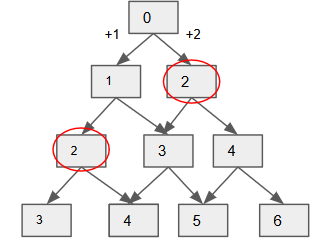
\includegraphics[width=0.6\columnwidth]{fig/min_climbing.png}
    \caption{Caption}
    \label{fig:min_climbing}
\end{figure}
Analysis: As Fig~\ref{fig:min_climbing} shows, the mincost to get 2 is only dependent on the mincost of 0, 1, each goes 2 and 1 steps respectively. To get 3, is only dependent on the mincost of 1, 2. For 0, 1, the cost is initialize as 0 because it is the starting point.
\begin{lstlisting}[language=Python]
def minCostClimbingStairs(self, cost):
    if not cost:
        return 0
    dp = [sys.maxsize]*(len(cost)+1)
    
    dp[0] = 0
    dp[1] = 0
    for i in range(2, len(cost)+1):
        dp[i] = min(dp[i], dp[i-1]+cost[i-1], dp[i-2]+cost[i-2])
    return dp[-1]
\end{lstlisting}


576. Out of Boundary Paths (Medium)
\begin{lstlisting}
There is an m by n grid with a ball. Given the start coordinate (i,j) of the ball, you can move the ball to adjacent cell or cross the grid boundary in four directions (up, down, left, right). However, you can at most move N times. Find out the number of paths to move the ball out of grid boundary. The answer may be very large, return it after mod 10^9 + 7.

Example 1:
Input: m = 2, n = 2, N = 2, i = 0, j = 0
Output: 6
Explanation:

Example 2:
Input: m = 1, n = 3, N = 3, i = 0, j = 1
Output: 12
Explanation:

Note:
    Once you move the ball out of boundary, you cannot move it back.
    The length and height of the grid is in range [1,50].
    N is in range [0,50].
\end{lstlisting}
\textbf{Multiple Time Coordinate}. The only difference compared with our examples, we track the out of boundary paths each time when the next location is not within bound. 
\begin{lstlisting}[language=Python]
def findPaths(self, m, n, N, i, j):
    MOD = 10**9+7
    dirs = [(-1, 0), (1, 0),(0, -1),(0, 1)]
    dp = [[0 for _ in range(n)] for _ in range(m)]
    dp[i][j] = 1
    ans = 0
    
    for step in range(N):
        new_dp = [[0 for _ in range(n)] for _ in range(m)]
        for x in range(m):
            for y in range(n):
                if dp[x][y] == 0: #only check available location at that step
                    continue
                for dx, dy in dirs:
                    nx, ny = x+dx, y+dy
                    if 0 <= nx < m and 0 <= ny < n:
                        new_dp[nx][ny] += dp[x][y]
                    else:
                        ans += dp[x][y]
                        ans %= MOD
        dp = new_dp
    
    return ans
\end{lstlisting}

63. Unique Paths II
\begin{lstlisting}
A robot is located at the top-left corner of a m x n grid (marked 'Start' in the diagram below).

The robot can only move either down or right at any point in time. The robot is trying to reach the bottom-right corner of the grid (marked 'Finish' in the diagram below).

Now consider if some obstacles are added to the grids. How many unique paths would there be?

An obstacle and empty space is marked as 1 and 0 respectively in the grid.

Note: m and n will be at most 100.

Example 1:

Input:
[
  [0,0,0],
  [0,1,0],
  [0,0,0]
]
Output: 2
Explanation:
There is one obstacle in the middle of the 3x3 grid above.
There are two ways to reach the bottom-right corner:
1. Right -> Right -> Down -> Down
2. Down -> Down -> Right -> Right
\end{lstlisting}
\textbf{Coordinate}. 
\begin{lstlisting}[language=Python]
def uniquePathsWithObstacles(self, obstacleGrid):
    """
    :type obstacleGrid: List[List[int]]
    :rtype: int
    """
    if not obstacleGrid or obstacleGrid[0][0] == 1:
        return 0
    m, n = len(obstacleGrid), len(obstacleGrid[0])
    dp = [[0 for c in range(n)] for r in range(m)]
    dp[0][0] = 1 if obstacleGrid[0][0] == 0 else 0 # starting point
    
    # init col
    for r in range(1, m):
        dp[r][0] = dp[r-1][0] if obstacleGrid[r][0] == 0 else 0
        
    for c in range(1, n):
        dp[0][c] = dp[0][c-1] if obstacleGrid[0][c] == 0 else 0
        
    for r in range(1, m):
        for c in range(1, n):
            dp[r][c] = dp[r-1][c] + dp[r][c-1] if obstacleGrid[r][c] == 0 else 0
    print(dp)
    return dp[-1][-1]
\end{lstlisting}


\subsection{Double Sequence}
712. Minimum ASCII Delete Sum for Two Strings
\begin{lstlisting}
Given two strings s1, s2, find the lowest ASCII sum of deleted characters to make two strings equal.

Example 1:

Input: s1 = "sea", s2 = "eat"
Output: 231
Explanation: Deleting "s" from "sea" adds the ASCII value of "s" (115) to the sum.
Deleting "t" from "eat" adds 116 to the sum.
At the end, both strings are equal, and 115 + 116 = 231 is the minimum sum possible to achieve this.

Example 2:

Input: s1 = "delete", s2 = "leet"
Output: 403
Explanation: Deleting "dee" from "delete" to turn the string into "let",
adds 100[d]+101[e]+101[e] to the sum.  Deleting "e" from "leet" adds 101[e] to the sum.
At the end, both strings are equal to "let", and the answer is 100+101+101+101 = 403.
If instead we turned both strings into "lee" or "eet", we would get answers of 433 or 417, which are higher.

Note:
0 < s1.length, s2.length <= 1000.
All elements of each string will have an ASCII value in [97, 122].
\end{lstlisting}

\begin{lstlisting}[language=Python]
def minimumDeleteSum(self, s1, s2):
    word1, word2=s1,s2
    if not word1:
        if not word2:
            return 0
        else:
            return sum([ord(c) for c in word2])
    if not word2:
        return sum([ord(c) for c in word1])
    
    rows, cols=len(word1),len(word2)
    
    dp = [[0 for col in range(cols+1)] for row in range(rows+1)]
    for i in range(1,rows+1):
        dp[i][0] = dp[i-1][0] + ord(word1[i-1]) #delete in word1
    for j in range(1,cols+1):
        dp[0][j] = dp[0][j-1] + ord(word2[j-1]) #delete in word2
        
    for i in range(1,rows+1):
        for j in range(1,cols+1):
            if word1[i-1] == word2[j-1]:
                dp[i][j] = dp[i-1][j-1]
            else:
                dp[i][j] = min(dp[i][j-1] + ord(word2[j-1]), dp[i-1][j] + ord(word1[i-1])) #delete in word2, delete in word1
    return dp[rows][cols]
\end{lstlisting}

\end{document}